\documentclass[11pt, a4paper]{article}
\usepackage[T1]{fontenc}
\usepackage[utf8]{inputenc}
\usepackage[top=0.85in, bottom=0.85in, left=0.85in, right=0.85in]{geometry}
\usepackage{helvet}
\renewcommand{\familydefault}{\sfdefault}
\usepackage{amsmath, amssymb}
\usepackage{graphicx}
\usepackage{float}
\usepackage{booktabs}
\usepackage{tabularx}
\usepackage{array}
\usepackage{xcolor}
\usepackage{caption}
\usepackage{enumitem}
\usepackage{setspace}
\usepackage{fancyhdr}
\usepackage{listings}
\usepackage{tikz}
\usetikzlibrary{arrows.meta, positioning, shapes.geometric}
\usepackage{cite}
\renewcommand{\citepunct}{], [}
\renewcommand{\citedash}{]--[}
\usepackage{hyperref}

\setstretch{1.10}
\setlength{\parskip}{0.4em}
\setlength{\parindent}{0pt}
\captionsetup{skip=6pt, font=small, labelfont=bf}
\setlist{itemsep=0.15em, topsep=0.25em}
\graphicspath{{../figures/}}

\hypersetup{
  colorlinks=true,
  linkcolor=blue!60!black,
  urlcolor=blue!60!black,
  citecolor=blue!60!black,
  pdftitle={DSA5205 Project 2, Group 28: Systematic Trading Strategies for NVIDIA (NVDA)}
}

\lstset{
  basicstyle=\ttfamily\scriptsize,
  breaklines=true,
  columns=fullflexible,
  frame=single,
  rulecolor=\color{black!25},
  xleftmargin=3pt,
  xrightmargin=3pt,
  showstringspaces=false
}

\pagestyle{fancy}
\fancyhf{}
\lhead{\small DSA5205 Project 2 $\cdot$ Group 28}
\rhead{\small Systematic Trading Strategies for NVIDIA (NVDA)}
\cfoot{\thepage}
\renewcommand{\headrulewidth}{0.4pt}

\newcolumntype{L}{>{\raggedright\arraybackslash}X}
\newcolumntype{C}{>{\centering\arraybackslash}X}
\newcolumntype{R}{>{\raggedleft\arraybackslash}X}

\begin{document}

% =====================================================================
% 1. TITLE PAGE
% =====================================================================
\begin{titlepage}
\centering
\vspace*{1.0in}
{\large\bfseries DSA5205 $\cdot$ PROJECT 2\par}
\vspace{0.35in}
\rule{\linewidth}{0.8pt}\\[0.25in]
{\LARGE\bfseries Systematic Trading Strategies for NVIDIA (NVDA)\par}
\vspace{0.12in}
{\Large Mean Reversion, Trend Following, and Volatility Targeting\par}
\vspace{0.22in}
\rule{\linewidth}{0.8pt}\\[0.55in]

{\Large\bfseries Group 28\par}
\vspace{0.25in}

\begin{table}[H]
\centering
\normalsize
\renewcommand{\arraystretch}{1.25}
\begin{tabular}{l l}
\toprule
\textbf{Name} & \textbf{Student ID} \\
\midrule
Diana & A0327258X \\
Marco & A0326704H \\
Poh Yu Jie & A0216055M \\
\bottomrule
\end{tabular}
\end{table}

\vfill
{\normalsize October 2026\par}
\end{titlepage}

% =====================================================================
% 2. TABLE OF CONTENTS
% =====================================================================
\newpage
\tableofcontents
\newpage

% =====================================================================
% 3. ABSTRACT
% =====================================================================
\section*{Abstract}
\addcontentsline{toc}{section}{Abstract}

This study evaluates whether systematic trading strategies can capture the long-term growth of NVIDIA Corporation (NVDA) while reducing the severe drawdowns associated with holding a single high-volatility stock. Between 2015 and 2023, NVDA's split-adjusted share price rose more than 100-fold, but passive investors endured drawdowns of $-56.0\%$ in 2018 and $-66.3\%$ in 2022. To address this risk-return trade-off, three systematic strategies are compared within a common backtesting framework: (1) short-term mean reversion using Ridge regression, (2) trend following using a 200-day simple moving average (SMA) filter alongside regularized momentum models, and (3) dynamic position sizing based on 20-day realized volatility.

All strategies are evaluated over an identical 80/20 chronological split covering 449 out-of-sample trading days from March 2022 to December 2023, net of a 10 basis point transaction cost. The 200-day SMA trend-following rule delivered the strongest performance, achieving a Sharpe ratio of 1.68, a compound annual growth rate (CAGR) of 70.36\%, and a maximum drawdown of $-19.30\%$, compared with a Sharpe ratio of 0.97 and a $-60.80\%$ drawdown for buy-and-hold NVDA. Volatility targeting at a 40\% annualized target also improved compounding efficiency, generating a 44.68\% CAGR (versus 42.28\% for buy-and-hold) while reducing maximum drawdown to $-42.45\%$. By contrast, daily mean reversion underperformed during the 2022 bear market because it repeatedly bought into a sustained decline, resulting in a Sharpe ratio of 0.85 and a $-59.40\%$ drawdown. Overall, the results show that simple regime filtering and volatility control were more effective than short-horizon return prediction for managing downside risk in NVDA during 2022--2023.

% =====================================================================
% 4. RESEARCH PROBLEM
% =====================================================================
\section{Research Problem}

\subsection{Why NVIDIA?}
NVIDIA Corporation (NASDAQ: NVDA) was one of the highest-performing US equities between 2 January 2015 and 29 December 2023. Driven by demand for graphics processing units (GPUs) in data centers and artificial intelligence infrastructure, NVDA's split- and dividend-adjusted share price increased by a factor of 102.5 over the 2,264-day sample, producing a full-sample annualized arithmetic return of 63.07\% and a compound annual growth rate (CAGR) of 67.45\%.

However, this long-term growth came with substantial volatility and deep losses during market downturns. Over the full 2015--2023 sample, NVDA had an annualized volatility of 48.16\%, compared with 18.10\% for the S\&P 500 ETF (SPY). As shown in Figure~\ref{fig:price_context}, passive investors experienced two major drawdowns: a $-56.0\%$ decline in late 2018 and a $-66.3\%$ decline between November 2021 and October 2022. A loss of 66.3\% requires a subsequent gain of 196.7\% simply to break even, making unmanaged single-stock exposure difficult to sustain in practice.

\begin{figure}[H]
\centering
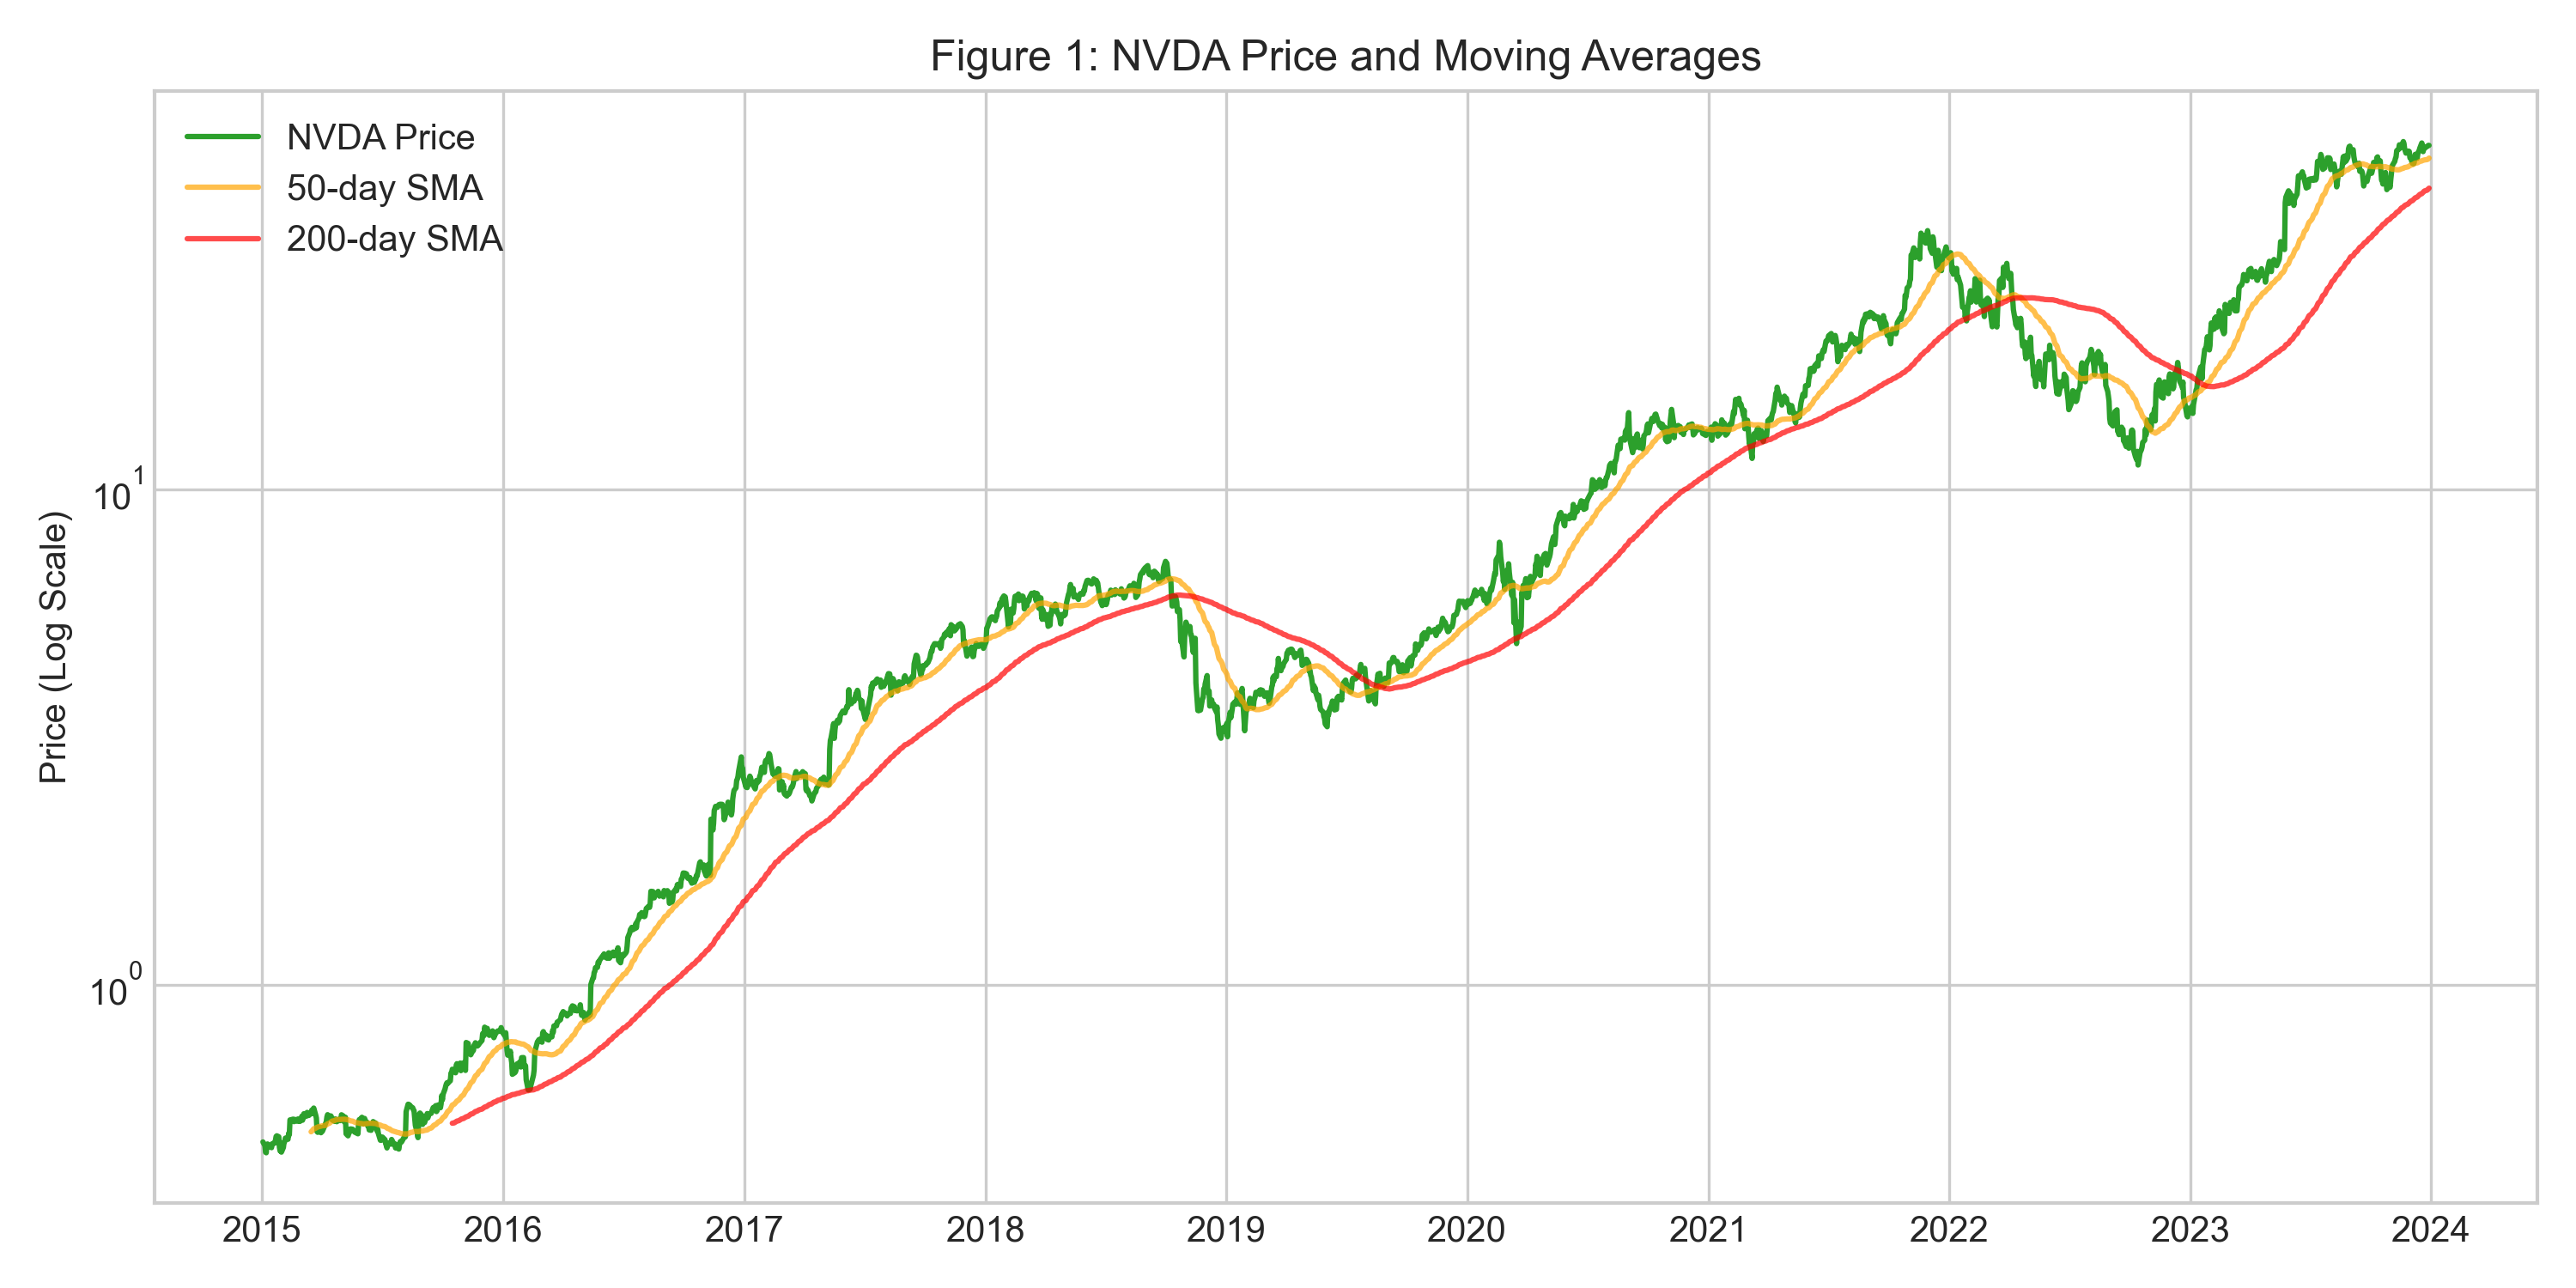
\includegraphics[width=0.82\textwidth, trim=0 25bp 0 0, clip]{eda_1_price.png}
\caption{Adjusted closing price of NVDA (log scale) with 50-day and 200-day simple moving averages from 2015 to 2023.}
\label{fig:price_context}
\end{figure}

\subsection{Research Question}
This trade-off between high long-term returns and severe intermediate losses motivates the central question of this study:

\begin{quote}
\textit{Can systematic trading strategies capture NVIDIA's long-term growth while reducing downside risk compared with simply buying and holding the stock?}
\end{quote}

\subsection{Research Hypotheses}
To evaluate this question, three hypotheses are tested, each corresponding to a distinct trading mechanism summarized in Table~\ref{tab:hypotheses}.

\begin{table}[H]
\centering
\small
\renewcommand{\arraystretch}{1.25}
\caption{Summary of Research Hypotheses.}
\label{tab:hypotheses}
\begin{tabularx}{\textwidth}{>{\raggedright\arraybackslash}p{4.0cm} >{\raggedright\arraybackslash}p{4.3cm} L}
\toprule
\textbf{Strategy} & \textbf{Economic Rationale} & \textbf{Hypothesis} \\
\midrule
\textbf{H1: Mean Reversion} & Short-term price declines may reverse & Ridge regression can identify profitable rebound opportunities \\
\textbf{H2: Trend Following} & Market trends may persist over time & A 200-day moving average can reduce losses during sustained declines \\
\textbf{H3: Volatility Targeting} & High volatility reduces compound growth & Adjusting exposure based on volatility can improve risk-adjusted performance \\
\bottomrule
\end{tabularx}
\end{table}

Formally, H1 tests whether $L_2$-regularized linear predictions trained on short-term return lags and moving-average distances can generate positive risk-adjusted returns after transaction costs. H2 tests whether conditioning equity exposure on a 200-day moving average filter (or regularized multi-horizon momentum) protects capital during extended downturns while preserving upside participation. H3 tests whether scaling portfolio weights inversely to 20-day realized volatility reduces variance drag and improves compound growth relative to passive buy-and-hold. Section~\ref{sec:method} details the methodology, Section~\ref{sec:results} presents the empirical results, Section~\ref{sec:discussion} examines the drivers and limitations of each strategy, and Section~\ref{sec:conclusion} evaluates the three hypotheses.

% =====================================================================
% 5. METHODOLOGY
% =====================================================================
\section{Methodology}
\label{sec:method}

\subsection{Research Framework}
To ensure a fair comparison, all strategies are evaluated using the same underlying price series, chronological train/test split, execution rules, and transaction cost assumptions. Figure~\ref{fig:pipeline_detailed} outlines the five-stage research workflow.

\begin{figure}[H]
\centering
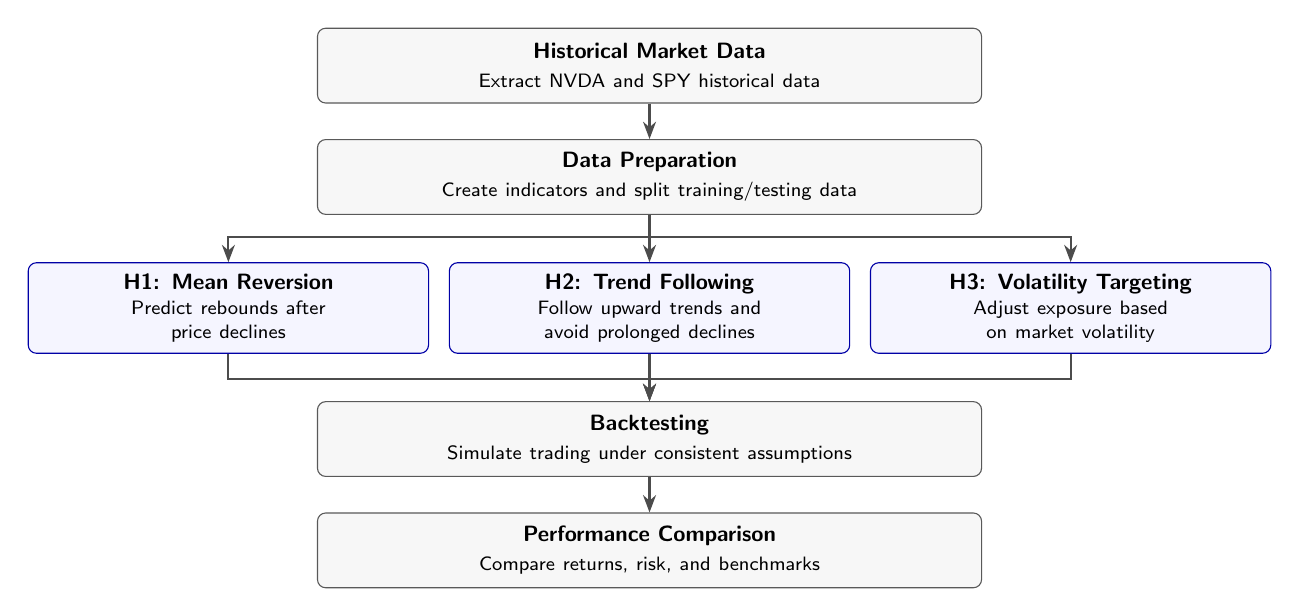
\begin{tikzpicture}[
  node distance=0.45cm and 0.30cm,
  flowbox/.style={draw=black!65, fill=black!3, rounded corners=3pt, align=center, font=\footnotesize, minimum height=0.95cm, text width=8.2cm},
  stratbox/.style={draw=blue!65!black, fill=blue!4, rounded corners=3pt, align=center, font=\footnotesize, minimum height=1.15cm, text width=4.85cm},
  arr/.style={-{Stealth[length=2.2mm]}, thick, draw=black!70}
]

\node[flowbox] (data) {\textbf{Historical Market Data}\\[1pt]{\scriptsize Extract NVDA and SPY historical data}};
\node[flowbox, below=0.45cm of data] (feat) {\textbf{Data Preparation}\\[1pt]{\scriptsize Create indicators and split training/testing data}};

\node[stratbox, below=0.6cm of feat] (h2) {\textbf{H2: Trend Following}\\[1pt]{\scriptsize Follow upward trends and\\[-1pt] avoid prolonged declines}};
\node[stratbox, left=0.25cm of h2] (h1) {\textbf{H1: Mean Reversion}\\[1pt]{\scriptsize Predict rebounds after\\[-1pt] price declines}};
\node[stratbox, right=0.25cm of h2] (h3) {\textbf{H3: Volatility Targeting}\\[1pt]{\scriptsize Adjust exposure based\\[-1pt] on market volatility}};

\node[flowbox, below=0.6cm of h2] (bt) {\textbf{Backtesting}\\[1pt]{\scriptsize Simulate trading under consistent assumptions}};
\node[flowbox, below=0.45cm of bt] (perf) {\textbf{Performance Comparison}\\[1pt]{\scriptsize Compare returns, risk, and benchmarks}};

\draw[arr] (data) -- (feat);
\draw[arr] (feat.south) -- ++(0,-0.28) -| (h1.north);
\draw[arr] (feat.south) -- (h2.north);
\draw[arr] (feat.south) -- ++(0,-0.28) -| (h3.north);
\draw[arr] (h1.south) |- ([yshift=0.28cm]bt.north) -- (bt.north);
\draw[arr] (h2.south) -- (bt.north);
\draw[arr] (h3.south) |- ([yshift=0.28cm]bt.north) -- (bt.north);
\draw[arr] (bt) -- (perf);

\end{tikzpicture}
\caption{Conceptual workflow of the research framework.}
\label{fig:pipeline_detailed}
\end{figure}

\subsection{Data and Trading Assumptions}
\label{sec:market}

The study focuses on NVIDIA Corporation (NVDA), priced in US Dollars (USD). Analyzing a single liquid large-cap stock isolates the time-series properties of the three strategies without introducing cross-sectional covariance estimation noise. Daily data from 2 January 2015 to 29 December 2023 (2,264 trading days) are retrieved from Yahoo Finance using \texttt{yfinance} (\texttt{src/data.py}). Because NVDA completed a 4-for-1 stock split on 20 July 2021, unadjusted prices would create an artificial $-75\%$ one-day return. All prices are therefore adjusted backward for splits and dividends using \texttt{auto\_adjust=True}:
\begin{equation}
A_t = P_t \cdot \prod_{s > t} g_s
\end{equation}
where $g_s$ is the adjustment factor for split ratios and dividend distributions. Trading days with missing values in either NVDA or SPY are removed.

To prevent look-ahead bias, the backtest separates historical signals from future returns:
\begin{enumerate}
    \item \textbf{Historical Feature Construction:} All signals, moving averages, and model predictions at day $t$ use only prices up to day $t$, $\mathcal{F}_t = \{P_s : s \le t\}$. The predicted return $R_{t+1} = (P_{t+1} - P_t)/P_t$ covers the next trading day $(t, t+1]$.
    \item \textbf{Same-Day Closing Price Assumption:} In the baseline backtest, portfolio weights $w_t$ determined at day $t$ are assumed to be executed at the closing price $P_t$, earning $w_t \cdot R_{t+1}$ over the following day, subject to a 10 basis point transaction cost.
    \item \textbf{Delayed Execution Sensitivity Check:} Because live market-on-close orders must be submitted shortly before the 16:00 EST closing auction, using the final closing price $P_t$ for both signal calculation and trade execution introduces a timing approximation. To test whether the findings depend on same-close execution, Section~\ref{sec:res_tradeoff} (Table~\ref{tab:lag_audit}) evaluates a strict one-day execution delay ($w_{t-1} \cdot R_{t+1}$).
\end{enumerate}

\subsection{Prediction Target and Features}
\label{sec:features}

All supervised learning models predict the next-day simple return:
\begin{equation}
y_t \equiv R_{t+1} = \frac{P_{t+1} - P_t}{P_t}
\end{equation}
implemented via \texttt{df['Return'].shift(-1)}. The final trading day has no next-day return and is excluded prior to data splitting. Table~\ref{tab:features_detailed} summarizes the 12 features and indicators used across the three strategies, comprising 10 regression predictors (6 for Strategy 1 and 4 for Strategies 2b/2c) and 2 rule-based reference indicators (\texttt{SMA\_200} for Strategy 2a and $\sigma_{t, 20\text{d}}$ for Strategy 3).

\begin{table}[H]
\centering
\small
\renewcommand{\arraystretch}{1.18}
\caption{Feature and Indicator Definitions Across Strategies.}
\label{tab:features_detailed}
\begin{tabularx}{\textwidth}{l p{4.2cm} L}
\toprule
\textbf{Feature / Indicator} & \textbf{Definition} & \textbf{Purpose} \\
\midrule
\multicolumn{3}{l}{\textit{Strategy 1: Mean Reversion (6 Regression Features)}} \\
\texttt{Ret\_0} & $P_t / P_{t-1} - 1$ & Captures same-day return shocks and sharp daily selloffs. \\
\texttt{Ret\_Lag1} & $P_{t-1} / P_{t-2} - 1$ & One-day lagged return measuring immediate follow-through. \\
\texttt{Ret\_Lag2} & $P_{t-2} / P_{t-3} - 1$ & Two-day lagged return capturing short-term return decay. \\
\texttt{Ret\_Lag5} & $P_{t-1} / P_{t-6} - 1$ & Prior five-day return measuring weekly price drift. \\
\texttt{Dist\_MA10} & $(P_t - \text{MA}_{10,t}) / \text{MA}_{10,t}$ & Percentage distance from the 10-day moving average (short-term dip signal). \\
\texttt{Dist\_MA20} & $(P_t - \text{MA}_{20,t}) / \text{MA}_{20,t}$ & Percentage distance from the 20-day moving average (medium-term dip signal). \\
\midrule
\multicolumn{3}{l}{\textit{Strategy 2: Trend Following (1 Rule Indicator + 4 Regression Features)}} \\
\texttt{SMA\_200} & $\frac{1}{200}\sum_{i=0}^{199} P_{t-i}$ & Reference 200-day moving average used by Strategy 2a to separate bull and bear regimes. \\
\texttt{Dist\_SMA50} & $(P_t - \text{SMA}_{50,t}) / \text{SMA}_{50,t}$ & Percentage distance from the 50-day moving average (Strategies 2b/2c). \\
\texttt{Dist\_SMA200} & $(P_t - \text{SMA}_{200,t}) / \text{SMA}_{200,t}$ & Percentage distance from the 200-day moving average (Strategies 2b/2c). \\
\texttt{Mom\_10d} & $P_t / P_{t-10} - 1$ & Two-week price momentum (Strategies 2b/2c). \\
\texttt{Mom\_20d} & $P_t / P_{t-20} - 1$ & One-month price momentum (Strategies 2b/2c). \\
\midrule
\multicolumn{3}{l}{\textit{Strategy 3: Volatility Targeting (1 Rule Indicator)}} \\
$\sigma_{t, 20\text{d}}$ & $\text{std}(R_{t-19 \dots t}) \times \sqrt{252}$ & Trailing 20-day annualized volatility used to scale position sizes. \\
\bottomrule
\end{tabularx}
\end{table}

Exploratory analysis (\texttt{scripts/split\_eda.py}) motivated these feature choices. Figure~\ref{fig:eda_zscore} shows the rolling 50-day price Z-score ($Z_t = (P_t - \mu_{50,t}) / \sigma_{50,t}$), where values below $-2.0$ mark sharp short-term selloffs. Figure~\ref{fig:eda_hurst} plots the 60-day rolling Hurst exponent ($H$)~\cite{hurst1951}, which fluctuates above and below $0.5$, indicating that NVDA alternates between trending ($H > 0.5$) and mean-reverting ($H < 0.5$) phases. To avoid overfitting, these exploratory indicators are not used as hard trading filters; instead, the strategies rely directly on the features in Table~\ref{tab:features_detailed}.

\begin{figure}[H]
\centering
\begin{minipage}[t]{0.48\textwidth}
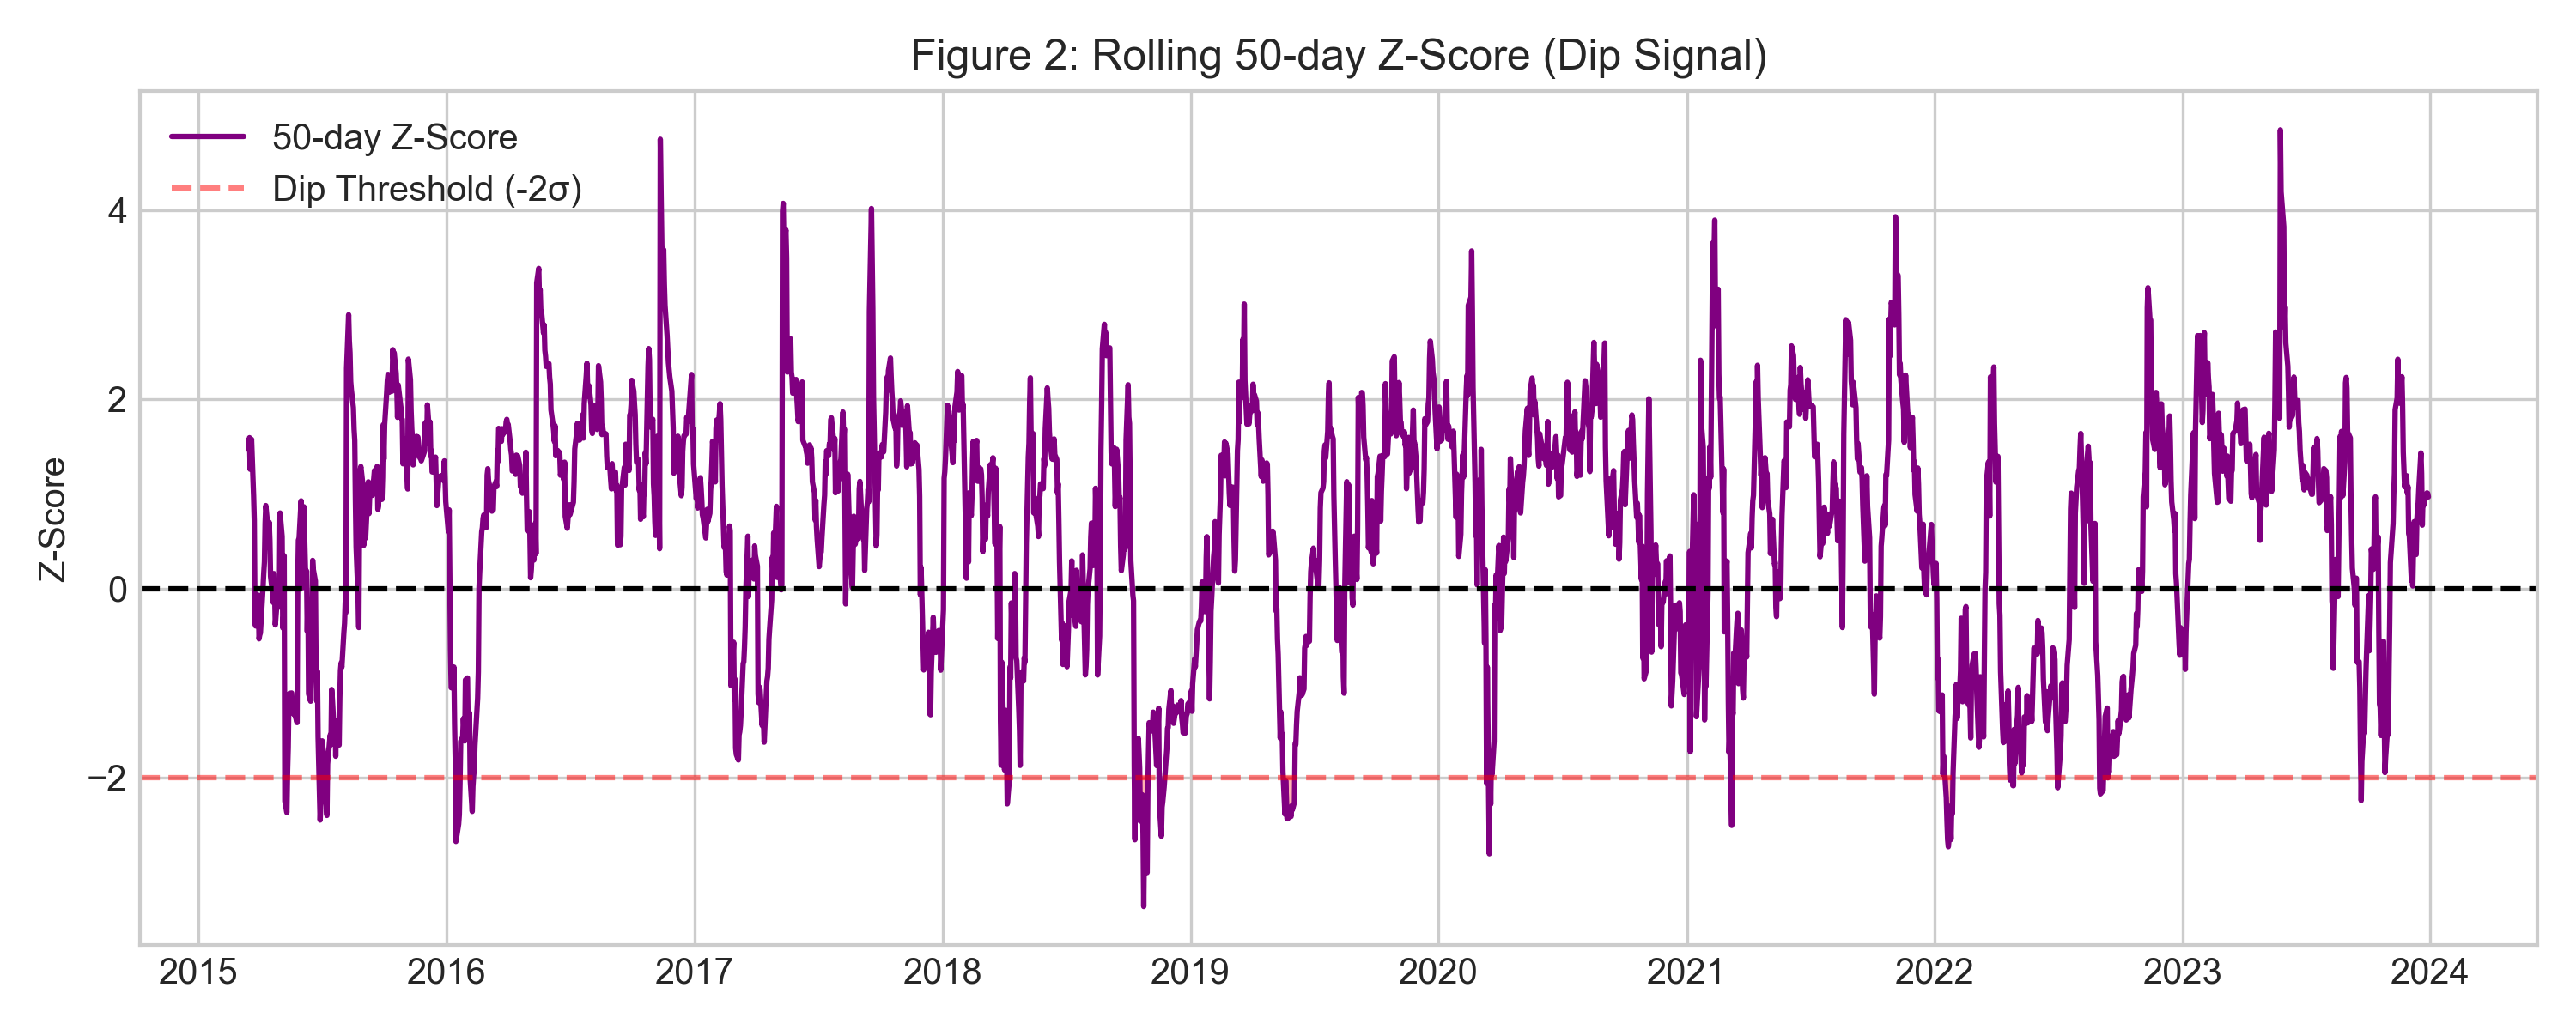
\includegraphics[width=\textwidth, trim=0 20bp 0 0, clip]{eda_2_zscore.png}
\caption{Rolling 50-day price Z-score of NVDA.}
\label{fig:eda_zscore}
\end{minipage}
\hfill
\begin{minipage}[t]{0.48\textwidth}
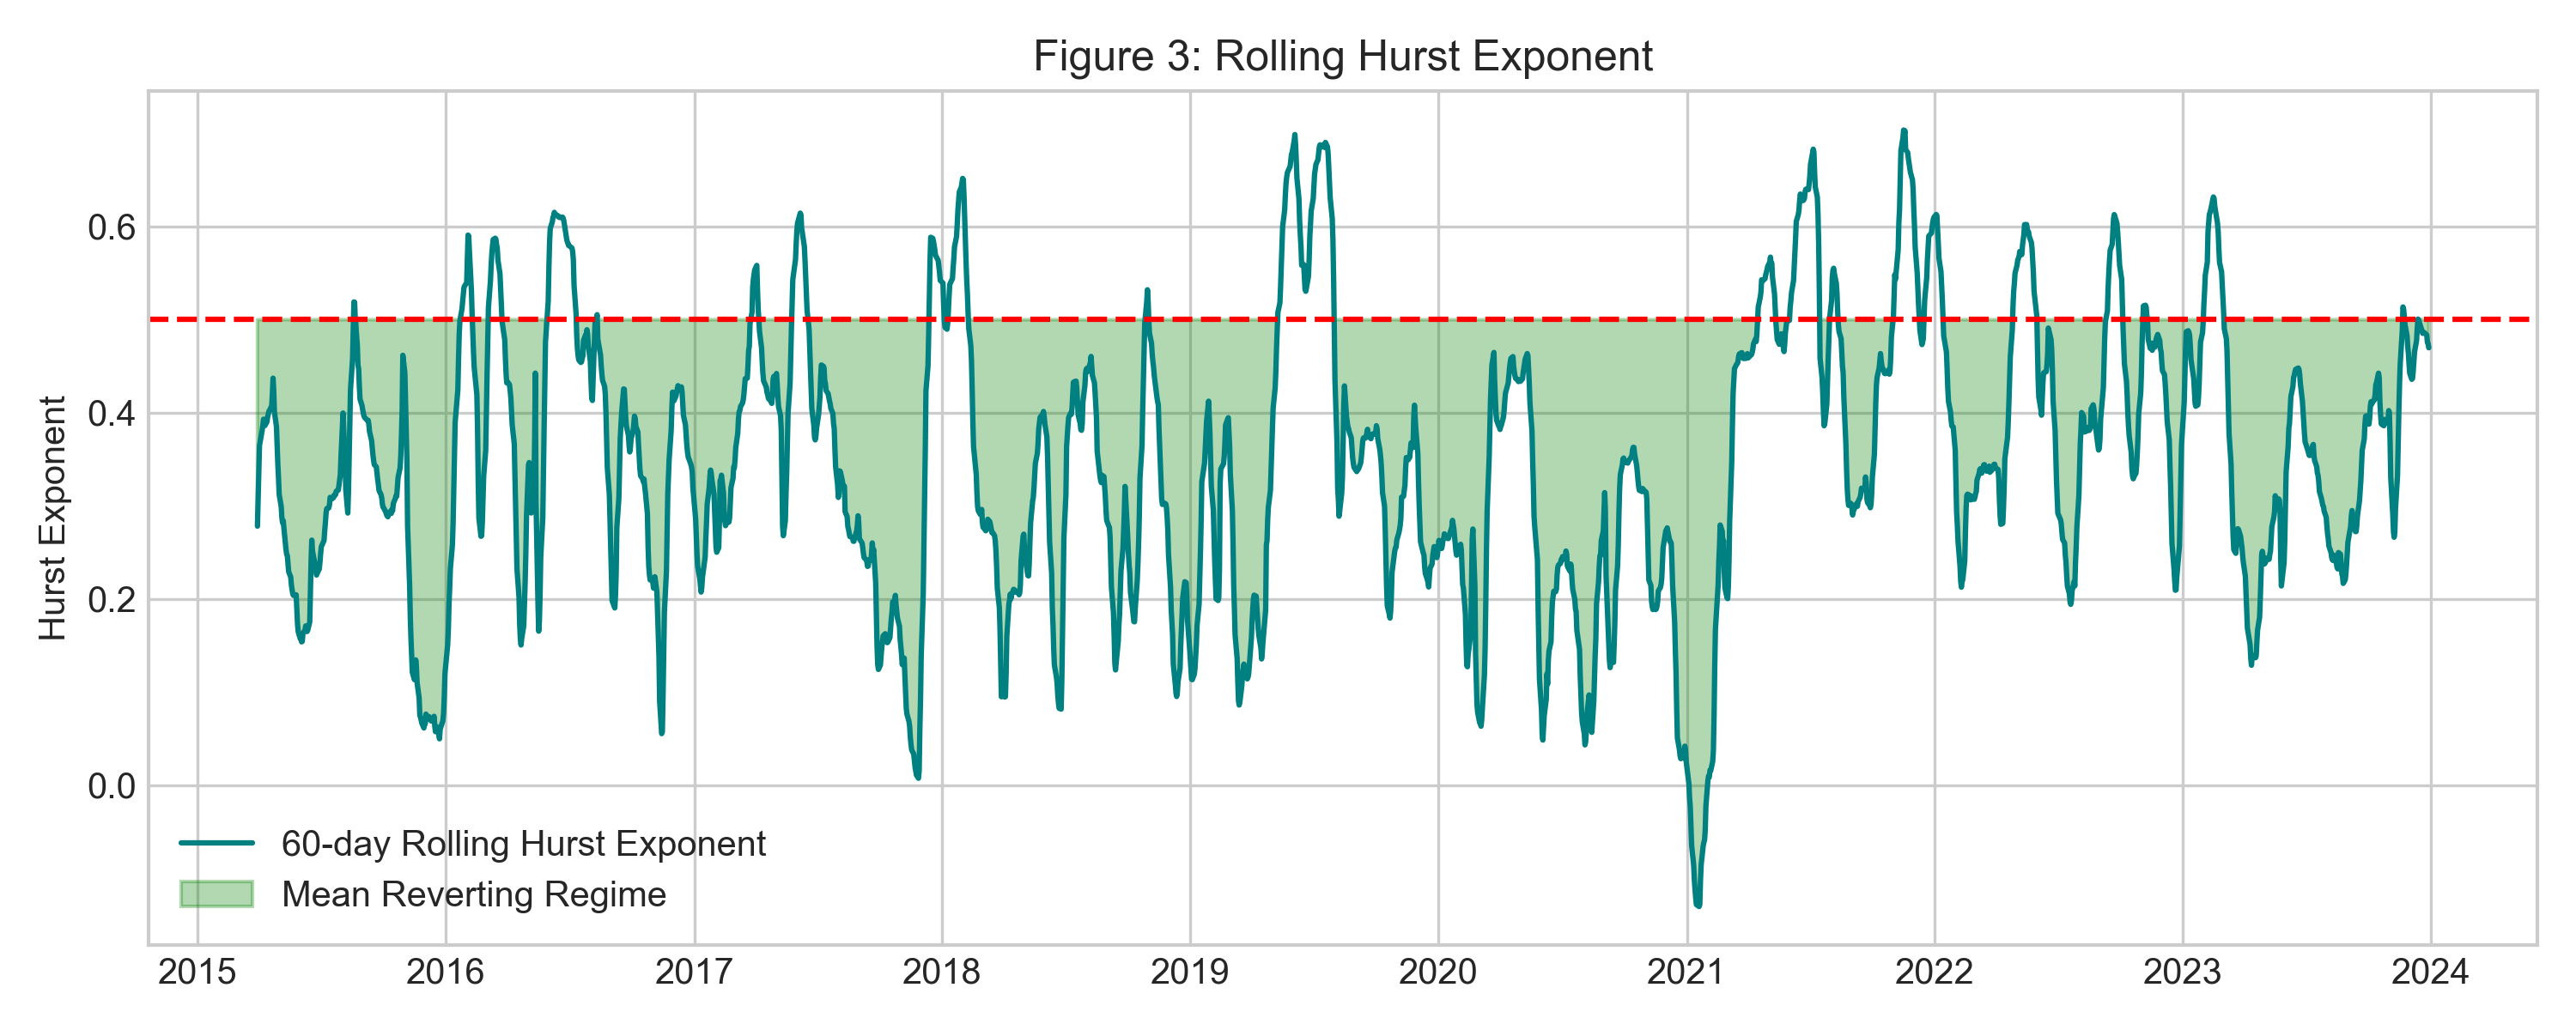
\includegraphics[width=\textwidth, trim=0 20bp 0 0, clip]{eda_3_hurst.png}
\caption{Rolling 60-day Hurst exponent of NVDA.}
\label{fig:eda_hurst}
\end{minipage}
\end{figure}

\subsection{Data Splitting and Leakage Prevention}
\label{sec:split}

Because financial time series are serially correlated and non-stationary, random cross-validation would leak future market conditions into the training set. After removing initial moving-average warm-up rows, the 2,244 trading days are divided chronologically into an 80/20 split:
\begin{itemize}
    \item \textbf{Training and Validation Set (80\%):} $T_{\text{train}} = 1,795$ trading days from 30 January 2015 to 16 March 2022, covering the 2018 semiconductor downturn, the 2020 COVID-19 selloff, and the 2021 bull market.
    \item \textbf{Out-of-Sample Test Set (20\%):} $T_{\text{test}} = 449$ trading days from 17 March 2022 to 28 December 2023, held out during model training and evaluated once for final comparison.
\end{itemize}

Because regularized regression penalizes coefficients based on scale, all features are standardized using only training-set statistics:
\begin{equation}
\mu_{\text{train}} = \frac{1}{T_{\text{train}}}\sum_{t=1}^{T_{\text{train}}} X_t, \quad \sigma_{\text{train}} = \sqrt{\frac{1}{T_{\text{train}}}\sum_{t=1}^{T_{\text{train}}} (X_t - \mu_{\text{train}})^2}
\end{equation}
Out-of-sample test features are standardized using these fixed training parameters:
\begin{equation}
X_{\text{test, scaled}} = \frac{X_{\text{test}} - \mu_{\text{train}}}{\sigma_{\text{train}}}
\end{equation}

\subsection{Benchmarks}
\label{sec:benchmarks}
Strategy performance is compared against three baselines:
\begin{enumerate}
    \item \textbf{NVDA Buy-and-Hold:} Investing 100\% in NVDA at the start of the test period and holding without rebalancing.
    \item \textbf{SPY ETF Buy-and-Hold:} Investing 100\% in the S\&P 500 ETF Trust over the same test window to represent a broad US equity benchmark.
    \item \textbf{Naive Return Forecasts:} Out-of-sample $R^2$ is measured against both a zero-return forecast and the historical training mean return~\cite{campbell2008}.
\end{enumerate}

\subsection{Strategy 1: Mean Reversion}
\label{sec:s1}

Short-term equity returns often exhibit negative autocorrelation over 1- to 20-day horizons as temporary selling pressure and overreaction reverse~\cite{jegadeesh1990, lehmann1990, lomackinlay1990}. Because short-term moving average distances such as \texttt{Dist\_MA10} and \texttt{Dist\_MA20} are highly correlated ($\rho = 0.871$ in the training set), ordinary least squares estimates suffer from high variance. Strategy 1 therefore uses Ridge regression ($L_2$ regularization) to shrink correlated coefficients toward zero~\cite{hoerl1970}:
\begin{equation}
\hat{\beta}^{\text{Ridge}} = \arg\min_{\beta_0, \beta} \left\{ \sum_{t=1}^{T} \left( y_t - \beta_0 - \sum_{j=1}^{p} \beta_j X_{t,j} \right)^2 + \alpha \sum_{j=1}^{p} \beta_j^2 \right\}
\end{equation}

The regularization parameter $\alpha$ is selected using a 5-fold expanding-window \texttt{TimeSeriesSplit} within the 80\% training set ($T_{\text{train}} = 1,795$). Within each fold, feature standardization is fitted only on the expanding training subset. Five candidate values are evaluated:
\begin{equation}
\alpha \in \{0.1, \ 1.0, \ 10.0, \ 100.0, \ 1000.0\}
\end{equation}
As shown in Table~\ref{tab:cv_results}, $\alpha = 1000.0$ achieved the highest mean validation $R^2$ because strong shrinkage limits overfitting on noisy daily returns.

\begin{table}[H]
\centering
\small
\caption{Strategy 1 Expanding-Window Cross-Validation Results.}
\label{tab:cv_results}
\begin{tabularx}{\textwidth}{c c L}
\toprule
\textbf{Regularization} ($\alpha$) & \textbf{Mean Validation} $R^2$ & \textbf{Interpretation} \\
\midrule
0.1 & $-0.01557$ & Weak shrinkage; high estimation noise \\
1.0 & $-0.01538$ & High coefficient variance \\
10.0 & $-0.01436$ & Moderate coefficient shrinkage \\
100.0 & $-0.01150$ & Stronger noise reduction \\
\textbf{1000.0 (Selected)} & $\mathbf{-0.00683}$ & \textbf{Strongest noise reduction; highest validation score} \\
\bottomrule
\end{tabularx}
\end{table}

Given the predicted next-day return $\hat{y}_t = \mathbb{E}[R_{t+1} | X_t]$, the strategy holds 100\% equity when the forecast is positive and moves to cash otherwise:
\begin{equation}
w_t^{\text{Ext1}} = \begin{cases} 1.0 & \text{if } \hat{y}_t > 0 \\ 0.0 & \text{if } \hat{y}_t \le 0 \end{cases}
\end{equation}

\subsection{Strategy 2: Trend Following}
\label{sec:s2}

While return reversals can occur over a few days, equity prices frequently trend over several months~\cite{moskowitz2012}. During prolonged downturns such as the 2022 technology selloff, buying short-term dips can lead to repeated losses as prices continue to fall. Strategy 2 evaluates whether medium- and long-term trend signals can avoid sustained bear markets.

The primary specification, \textbf{Strategy 2a}, uses a standard 200-day simple moving average (SMA) rule~\cite{faber2007} with no fitted parameters:
\begin{equation}
\text{SMA}_{200,t} = \frac{1}{200}\sum_{i=0}^{199} P_{t-i}
\end{equation}
\begin{equation}
w_t^{\text{Ext2a}} = \begin{cases} 1.0 & \text{if } P_t > \text{SMA}_{200,t} \quad \text{(100\% Equity)} \\ 0.0 & \text{if } P_t \le \text{SMA}_{200,t} \quad \text{(100\% Cash)} \end{cases}
\end{equation}

To test whether regression models can improve upon this simple rule, two machine learning variants are trained on four momentum indicators (\texttt{Dist\_SMA50}, \texttt{Dist\_SMA200}, \texttt{Mom\_10d}, and \texttt{Mom\_20d}):
\begin{itemize}
    \item \textbf{Strategy 2b (Ridge Momentum):} $L_2$-regularized linear regression ($\alpha = 10.0$)~\cite{hoerl1970}.
    \item \textbf{Strategy 2c (Lasso Momentum):} $L_1$-regularized sparse regression ($\alpha = 10^{-5}$)~\cite{tibshirani1996, chinco2019}.
\end{itemize}
Both models hold 100\% equity when the predicted return exceeds the training-set mean return ($\bar{y}_{\text{train}} = 0.267\%$) and hold cash otherwise.

\subsection{Strategy 3: Volatility Targeting}
\label{sec:s3}

Strategies 1 and 2 make binary allocation decisions ($w_t \in \{0.0, 1.0\}$). However, stock return volatility clusters in time~\cite{mandelbrot1963, engle1982}, and high-volatility periods erode compound returns through variance drag~\cite{moreira2017, harvey2018}:
\begin{equation}
g \approx \mu - \frac{1}{2}\sigma^2
\end{equation}
Strategy 3 adjusts position sizes continuously based on trailing 20-day annualized volatility:
\begin{equation}
\sigma_{t, 20\text{d}} = \sqrt{\frac{252}{19}\sum_{i=0}^{19}\left( R_{t-i} - \bar{R}_{t,20\text{d}} \right)^2}
\end{equation}
The baseline strategy sets an annualized target volatility of $\sigma_{\text{target}} = 0.40$ (40\%), chosen as a moderate risk budget slightly below NVDA's training-period volatility of roughly 45\%:
\begin{equation}
w_t^{\text{Ext3}} = \min\left(1.0, \ \frac{\sigma_{\text{target}}}{\max(\sigma_{t, 20\text{d}}, 10^{-6})}\right)
\end{equation}
Capping weights at 1.0 enforces a long-only, unleveraged constraint ($w_t \in [0.0, 1.0]$). When 20-day realized volatility rises above 40\%, the strategy reduces equity exposure; when volatility falls below 40\%, exposure returns to 100\%. Section~\ref{sec:res_ablation} examines sensitivity across alternative target levels from 20\% to 60\%.

\subsection{Trading Rules and Evaluation Metrics}
\label{sec:costs}

Each portfolio change incurs a transaction cost of 10 basis points (0.10\%) proportional to daily turnover:
\begin{equation}
\Delta w_t = |w_t - w_{t-1}|, \qquad R_{t+1}^{\text{net}} = \left( w_t \cdot R_{t+1} \right) - \left( \Delta w_t \times 0.0010 \right)
\end{equation}
A 10 bps cost accounts for bid-ask spreads (1--2 bps), clearing fees (0.5 bps), and market impact (about 7.5 bps) in a liquid large-cap stock.

Starting from initial capital $W_0 = \$100,000$, portfolio wealth evolves as $W_{t+1} = W_t (1 + R_{t+1}^{\text{net}})$. Over the $N = 449$ out-of-sample trading days, performance is evaluated using six metrics:
\begin{itemize}
    \item \textbf{Annualized Return:} $R_{\text{ann}} = \frac{252}{N} \sum_{t=1}^{N} R_t^{\text{net}}$
    \item \textbf{Compound Annual Growth Rate (CAGR):} $\text{CAGR} = \left(W_N / W_0\right)^{252/N} - 1$
    \item \textbf{Annualized Volatility:} $\sigma_{\text{ann}} = \text{std}(R_t^{\text{net}}) \times \sqrt{252}$
    \item \textbf{Sharpe Ratio ($R_f = 0$)~\cite{sharpe1994}:} $\text{Sharpe} = R_{\text{ann}} / \sigma_{\text{ann}}$
    \item \textbf{Maximum Drawdown:} $\text{MaxDD} = \min_{t} \left( \frac{W_t - \max_{s \le t} W_s}{\max_{s \le t} W_s} \right)$
    \item \textbf{Annualized Turnover:} $\text{Turnover} = \frac{252}{N} \sum_{t=1}^{N} |\Delta w_t|$
\end{itemize}
Note that $R_{\text{ann}}$ uses linear annualization ($252 \bar{R}_t$), whereas $\text{CAGR}$ compounds the daily geometric mean return $g_d = (W_N/W_0)^{1/N}-1$ via $(1+g_d)^{252}-1$. At the daily level, $g_d$ is always lower than $\bar{R}_t$ due to variance drag ($\bar{R}_t - g_d \approx \frac{1}{2}\sigma_d^2$), but when annual returns are high, 252-day exponential compounding in $\text{CAGR}$ can exceed linear scaling in $R_{\text{ann}}$ (as seen for full-sample NVDA and Strategy 2a).

\subsection{Reproducibility}
\label{sec:repro}
All experiments are implemented in Python 3.14.6 using NumPy 2.5.4, pandas 3.0.6, and the scikit-learn 1.9.1 library~\cite{pedregosa2011}. All random seeds are fixed at 42 (\texttt{random\_state=42}, \texttt{max\_iter=10000}), and every table and figure is reproduced by running:
\begin{center}
\texttt{scripts/run\_consolidated\_showdown.py}
\end{center}

% =====================================================================
% 6. RESULTS
% =====================================================================
\section{Results}
\label{sec:results}

Across the 449 out-of-sample trading days from 17 March 2022 to 28 December 2023 (net of 10 bps transaction costs), the simple 200-day moving average rule (Strategy 2a) outperformed both the machine learning models and passive buy-and-hold investing. By moving to cash during the 2022 downturn, Strategy 2a achieved a Sharpe ratio of 1.68, a CAGR of 70.36\%, and a maximum drawdown of $-19.30\%$, compared with a Sharpe ratio of 0.97 and a $-60.80\%$ drawdown for NVDA buy-and-hold. Volatility targeting at 40\% (Strategy 3) also improved compound growth over buy-and-hold (44.68\% vs.\ 42.28\% CAGR) while reducing maximum drawdown to $-42.45\%$. By contrast, daily mean reversion (Strategy 1) remained heavily exposed during the 2022 decline and experienced a $-59.40\%$ drawdown.

\subsection{Prediction Accuracy}
\label{sec:res_accuracy}

Table~\ref{tab:oos_accuracy} reports out-of-sample forecasting performance for the three regression models.

\begin{table}[H]
\centering
\small
\caption{Out-of-Sample Forecast Accuracy (449 Test Days).}
\label{tab:oos_accuracy}
\begin{tabularx}{\textwidth}{l C C C}
\toprule
\textbf{Model} & \textbf{OOS} $R^2$ \textbf{(vs.\ Zero)} & \textbf{OOS} $R^2$ \textbf{(vs.\ Mean)} & \textbf{Days Long} \\
\midrule
Strategy 1: Ridge Mean Reversion & $-0.00245$ & $-0.00603$ & 92.0\% \\
Strategy 2b: Ridge Momentum & $+0.00210$ & $-0.00140$ & 50.3\% \\
Strategy 2c: Lasso Momentum & $+0.00210$ & $-0.00150$ & 50.6\% \\
\bottomrule
\end{tabularx}
\end{table}

Because daily stock returns have a very low signal-to-noise ratio, out-of-sample $R^2$ values are close to zero across all three models~\cite{campbell2008, fama1970}. For Strategy 1, heavy regularization ($\alpha = 1000.0$) shrinks the slope coefficients toward zero, leaving predictions dominated by the positive training-set mean return ($+0.264\%$). As a result, Strategy 1 predicts a positive return on 92.0\% of test days.

Table~\ref{tab:learned_coefs} shows the fitted coefficients for Strategy 1 (\texttt{src/model.py}). The negative coefficients on \texttt{Ret\_0}, \texttt{Dist\_MA10}, and \texttt{Dist\_MA20} confirm the expected mean-reversion relationship: when NVDA falls below its short-term moving averages, the model predicts a higher next-day return.

\begin{table}[H]
\centering
\small
\caption{Strategy 1 Ridge Regression Coefficients ($\alpha = 1000.0$).}
\label{tab:learned_coefs}
\begin{tabularx}{\textwidth}{l c L}
\toprule
\textbf{Feature} & \textbf{Coefficient} ($\hat{\beta}$) & \textbf{Economic Interpretation} \\
\midrule
\texttt{Ret\_0} & $-0.001530$ & Negative weight: sharp daily declines increase predicted next-day return. \\
\texttt{Dist\_MA20} & $-0.000358$ & Negative weight: trading below the 20-day average signals an oversold dip. \\
\texttt{Dist\_MA10} & $-0.000226$ & Negative weight: trading below the 10-day average supports short-term rebound. \\
\texttt{Ret\_Lag5} & $-0.000093$ & Small negative weight: mild weekly reversal effect. \\
\texttt{Ret\_Lag2} & $+0.000547$ & Positive weight: short-term return persistence at a two-day lag. \\
\texttt{Ret\_Lag1} & $+0.000571$ & Positive weight: one-day return continuation. \\
\bottomrule
\end{tabularx}
\end{table}

\subsection{Strategy Performance Comparison}
\label{sec:res_showdown}

Table~\ref{tab:master_showdown} compares out-of-sample risk and return metrics across all five strategy variants and both benchmarks over the 449 test days.

\begin{table}[H]
\centering
\footnotesize
\setlength{\tabcolsep}{2.5pt}
\caption{Out-of-Sample Strategy Performance Comparison (449 Test Days, 2022--2023, Net of 10 bps Costs).}
\label{tab:master_showdown}
\begin{tabularx}{\textwidth}{l R R R R R R R}
\toprule
\textbf{Strategy / Benchmark} & \textbf{Ann.\ Ret} & \textbf{CAGR} & \textbf{Ann.\ Vol} & \textbf{Sharpe} & \textbf{MaxDD} & \textbf{Turnover} & \textbf{Final Wealth} \\
\midrule
Strategy 1: Mean Reversion (Ridge) & 45.96\% & 32.31\% & 54.06\% & 0.85 & $-59.40\%$ & 39.85 & \$175,738 \\
\textbf{Strategy 2a: 200-Day SMA Trend} & \textbf{63.83\%} & \textbf{70.36\%} & \textbf{37.88\%} & \textbf{1.68} & \textbf{-19.30\%} & \textbf{2.81} & \textbf{\$275,699} \\
Strategy 2b: Ridge Momentum & 12.19\% & 3.39\% & 42.67\% & 0.29 & $-48.35\%$ & 30.31 & \$106,113 \\
Strategy 2c: Lasso Momentum & 14.20\% & 5.56\% & 42.52\% & 0.33 & $-44.61\%$ & 29.18 & \$110,117 \\
\textbf{Strategy 3: Volatility Targeting (40\%)} & 47.63\% & 44.68\% & 42.14\% & 1.13 & $-42.45\%$ & 5.10 & \$200,316 \\
\midrule
\textit{NVDA Buy \& Hold Benchmark} & 54.06\% & 42.28\% & 55.49\% & 0.97 & $-60.80\%$ & 0.00 & \$200,201 \\
\textit{SPY ETF Benchmark} & 7.78\% & 5.48\% & 19.18\% & 0.41 & $-22.09\%$ & 0.00 & \$111,176 \\
\bottomrule
\end{tabularx}
\end{table}

Three findings stand out from Table~\ref{tab:master_showdown}:
\begin{itemize}
    \item \textbf{Trend Following Outperformance:} Strategy 2a achieved the highest risk-adjusted return, with a Sharpe ratio of 1.68, a CAGR of 70.36\%, and a maximum drawdown of $-19.30\%$.
    \item \textbf{Reduced Volatility Drag:} Strategy 3 generated a higher CAGR than NVDA Buy \& Hold (44.68\% vs.\ 42.28\%) while lowering annualized volatility by 13.35 percentage points and cutting maximum drawdown from $-60.80\%$ to $-42.45\%$.
    \item \textbf{Low-Turnover Advantage:} Strategy 2a had an annualized turnover of 2.81 (costing about 0.28\% per year), whereas Strategy 1's turnover of 39.85 reduced annual returns by roughly 3.99\%.
\end{itemize}

Figure~\ref{fig:showdown_equity} plots cumulative portfolio wealth on a logarithmic scale, and Figure~\ref{fig:showdown_dd} shows the corresponding underwater drawdown profiles.

\begin{figure}[H]
\centering
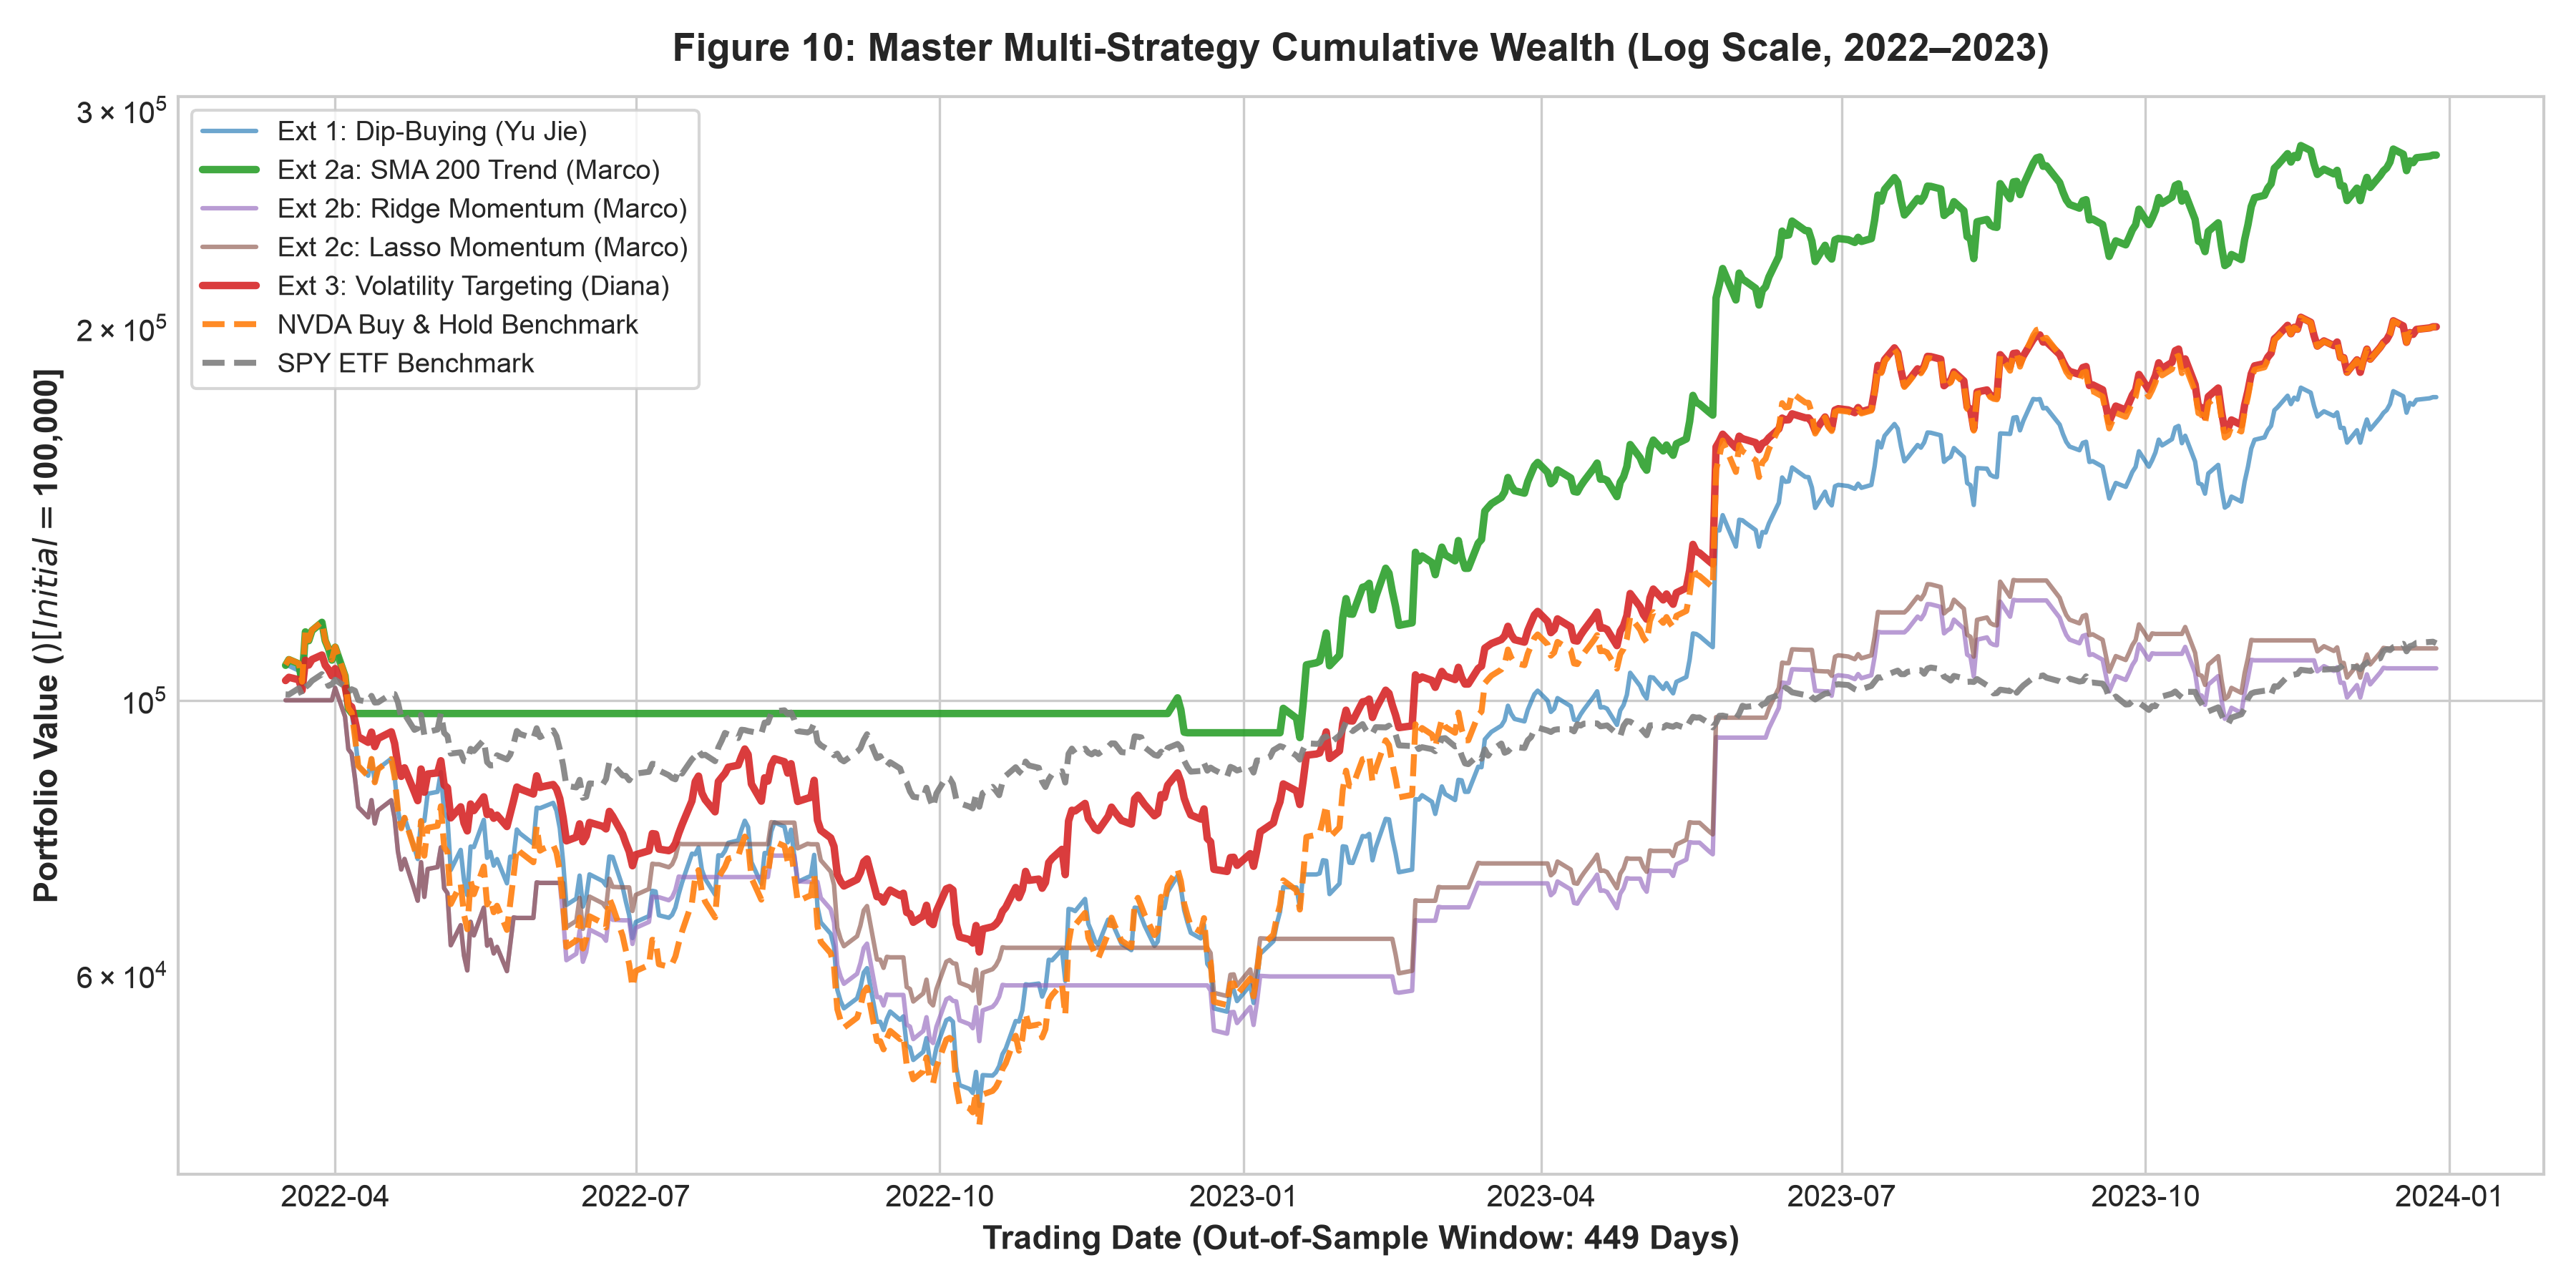
\includegraphics[width=0.82\textwidth, trim=0 26bp 0 0, clip]{consolidated_showdown_equity.png}
\caption{Out-of-sample cumulative wealth trajectories (\$100,000 initial capital, log scale, net of 10 bps costs).}
\label{fig:showdown_equity}
\end{figure}

\begin{figure}[H]
\centering
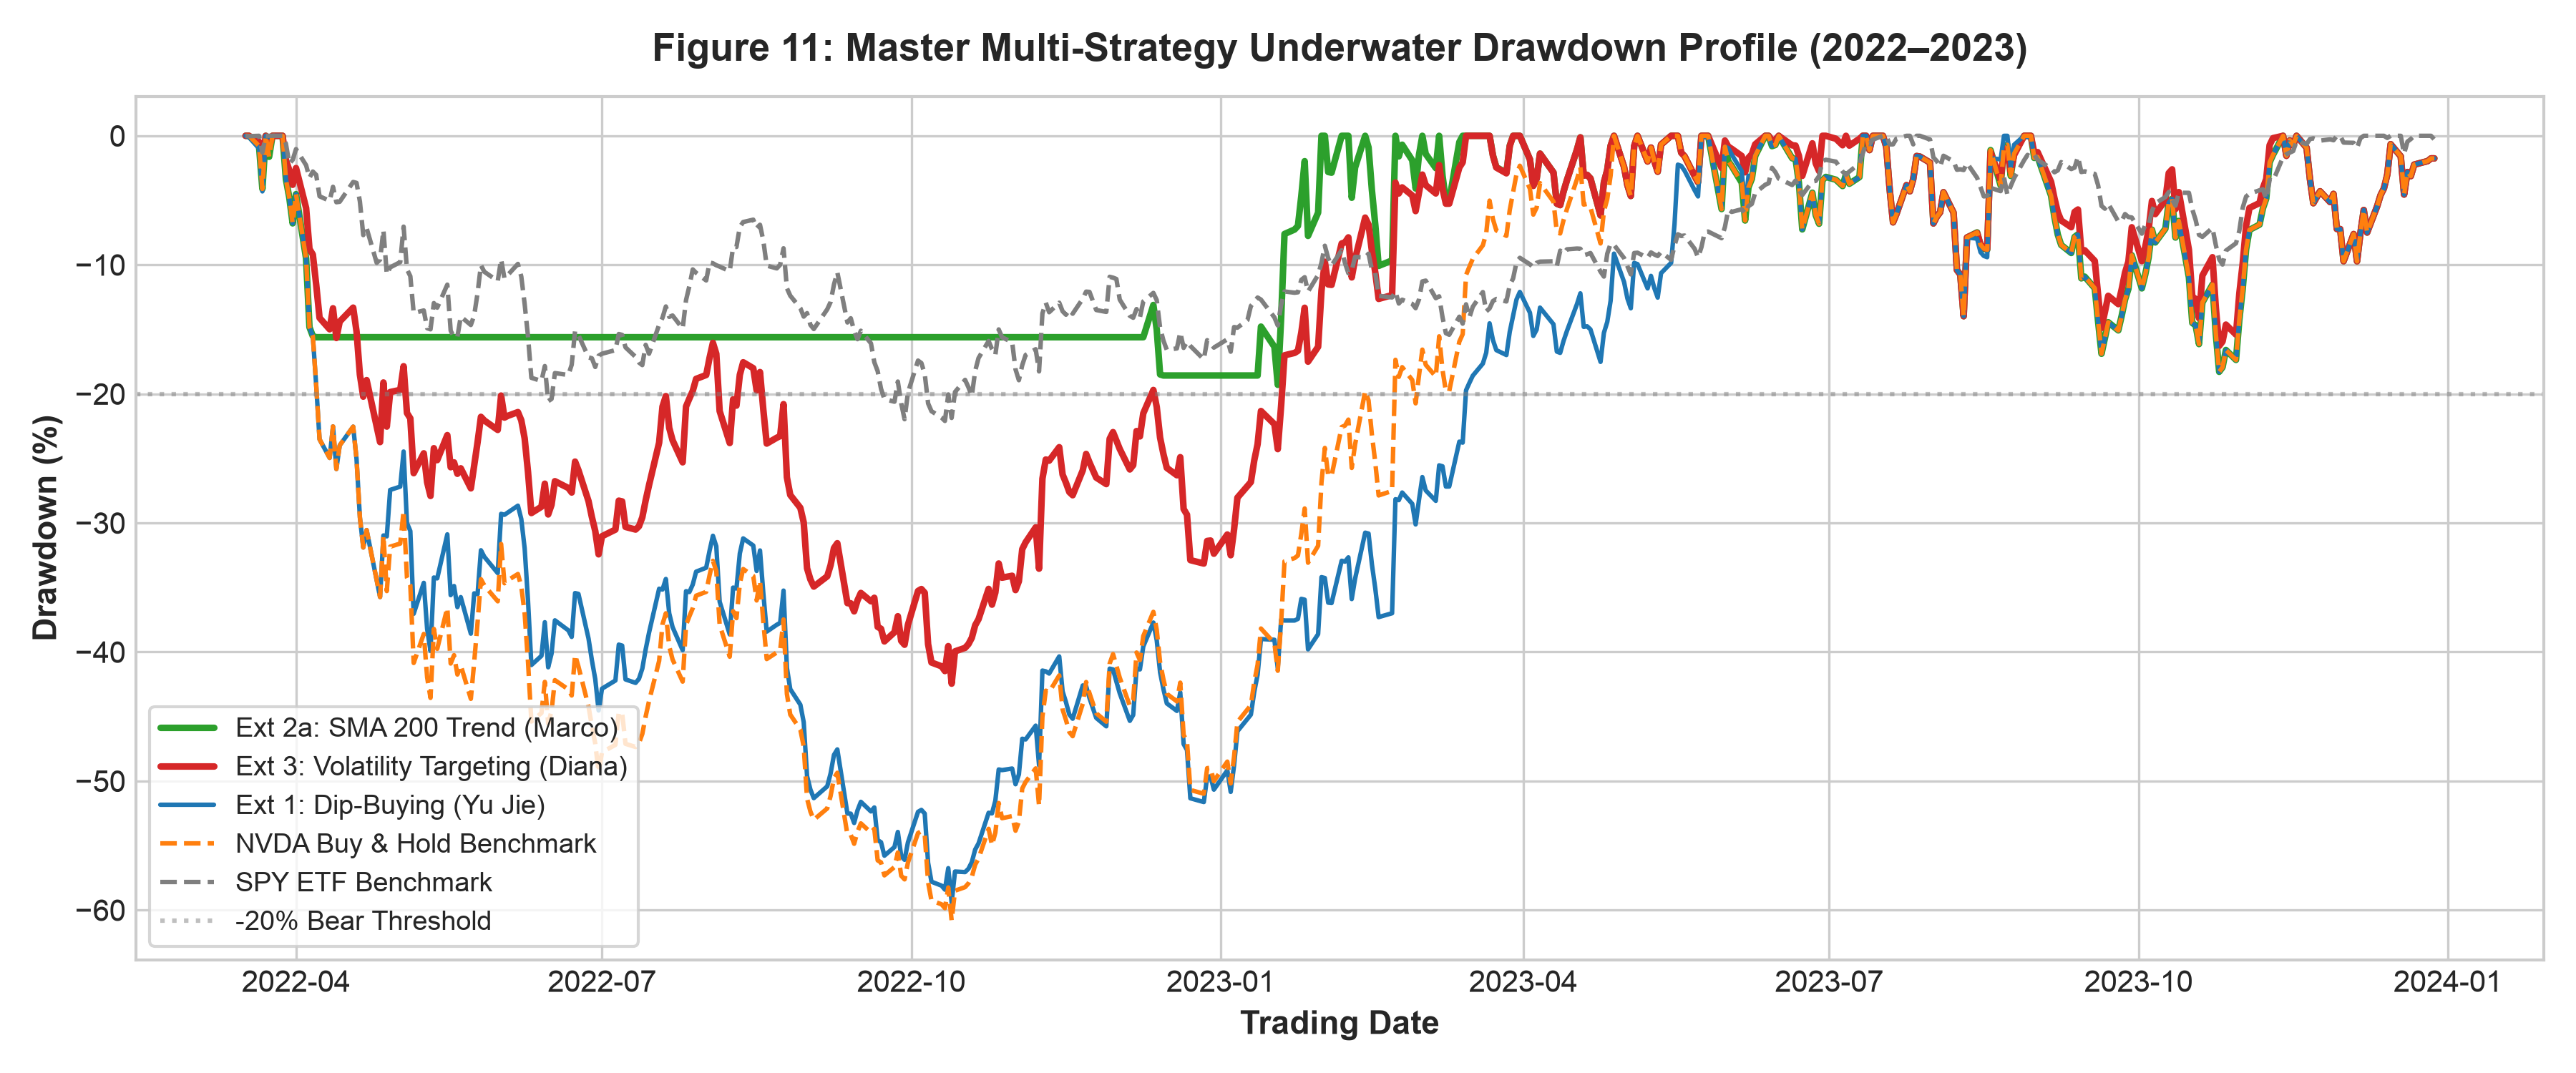
\includegraphics[width=0.82\textwidth, trim=0 26bp 0 0, clip]{consolidated_showdown_drawdown.png}
\caption{Out-of-sample drawdown profiles from March 2022 to December 2023.}
\label{fig:showdown_dd}
\end{figure}

\subsection{Performance in Bear and Bull Markets}
\label{sec:res_regimes}

The 449-day test period spans two distinct market environments: the 2022 technology bear market and the 2023 recovery. Table~\ref{tab:subperiod} reports performance in each sub-period.

\begin{table}[H]
\centering
\small
\setlength{\tabcolsep}{4.5pt}
\caption{Strategy Performance in the 2022 Bear Market and 2023 Bull Market.}
\label{tab:subperiod}
\begin{tabularx}{\textwidth}{l R R R R}
\toprule
& \multicolumn{2}{c}{\textbf{2022 Bear Market (200 Days)}} & \multicolumn{2}{c}{\textbf{2023 Bull Market (249 Days)}} \\
\cmidrule(lr){2-3} \cmidrule(lr){4-5}
\textbf{Strategy / Benchmark} & \textbf{Total Return} & \textbf{Sharpe Ratio} & \textbf{Total Return} & \textbf{Sharpe Ratio} \\
\midrule
Strategy 1: Mean Reversion (Ridge) & $-42.86\%$ & $-0.85$ & $+207.57\%$ & 2.64 \\
Strategy 2a: 200-Day SMA Trend & $\mathbf{-5.87\%}$ & $\mathbf{-0.31}$ & $+192.90\%$ & 2.51 \\
Strategy 2b: Ridge Momentum & $-45.15\%$ & $-1.42$ & $+93.46\%$ & 1.87 \\
Strategy 2c: Lasso Momentum & $-41.18\%$ & $-1.25$ & $+87.20\%$ & 1.78 \\
Strategy 3: Volatility Targeting (40\%) & $-26.45\%$ & $-0.72$ & $+172.35\%$ & 2.61 \\
\midrule
\textit{NVDA Buy \& Hold Benchmark} & $-42.15\%$ & $-0.79$ & $\mathbf{+246.10\%}$ & \textbf{2.83} \\
\textit{SPY ETF Benchmark} & $-12.26\%$ & $-0.54$ & $+26.71\%$ & 1.90 \\
\bottomrule
\end{tabularx}
\end{table}

Table~\ref{tab:subperiod} shows that Strategy 2a's advantage came from capital preservation in 2022. By moving to cash on 7 April 2022, Strategy 2a limited its 2022 loss to $-5.87\%$, whereas Buy \& Hold lost $-42.15\%$. During the 2023 rally, unhedged Buy \& Hold achieved the highest gain (+246.10\%), illustrating the opportunity cost of cash filters during rapid recoveries.

\subsection{Sensitivity to Training Period}
\label{sec:res_ext2_standalone}

In the standalone trend module (\texttt{scripts/run\_extension2\_momentum.py}), the 80/20 split is taken after removing the 200-day moving average warm-up period ($N = 2,064$ active days), producing a 413-day test window from 9 May 2022 to 28 December 2023. Table~\ref{tab:ext2_standalone} reports the resulting performance.

\begin{table}[H]
\centering
\small
\setlength{\tabcolsep}{3.5pt}
\caption{Strategy 2 Performance Under the 413-Day Split (May 2022 to December 2023).}
\label{tab:ext2_standalone}
\begin{tabularx}{\textwidth}{l R R R R}
\toprule
\textbf{Model} & \textbf{Ann.\ Return} & \textbf{Ann.\ Volatility} & \textbf{Sharpe Ratio} & \textbf{Max Drawdown} \\
\midrule
\textbf{Strategy 2a: 200-Day SMA Trend} & \textbf{70.15\%} & \textbf{37.50\%} & \textbf{1.87} & \textbf{-18.29\%} \\
Strategy 2c: Lasso Momentum & 63.64\% & 36.92\% & 1.72 & $-18.29\%$ \\
Strategy 2b: Ridge Momentum & 62.27\% & 37.62\% & 1.66 & $-18.29\%$ \\
\midrule
\textit{NVDA Buy \& Hold Benchmark} & 79.71\% & 53.84\% & 1.48 & $-42.67\%$ \\
\textit{SPY ETF Benchmark} & 14.43\% & 18.49\% & 0.78 & $-16.68\%$ \\
\bottomrule
\end{tabularx}
\end{table}

When the training period includes the March--April 2022 breakdown, the Ridge and Lasso momentum models (2b and 2c) assign a positive coefficient to \texttt{Dist\_SMA200} ($+0.000782$), stay in cash during the 2022 decline, and achieve Sharpe ratios of 1.66 and 1.72. When the split boundary begins 36 trading days earlier in Table~\ref{tab:master_showdown}, the training set ends before the regime break, causing the fitted momentum models to underperform. By contrast, the parameter-free 200-day SMA rule performs consistently across both split dates.

\subsection{Volatility Target Sensitivity}
\label{sec:res_ablation}

Figure~\ref{fig:ext3_alloc} shows how Strategy 3 adjusted its equity weight over the test period. When 20-day realized volatility rose to 86\% during the 2022 downturn, the portfolio weight fell to 45\%. After NVDA's 24.4\% one-day earnings gain on 25 May 2023 pushed trailing volatility to 95.5\%, exposure briefly decreased to 42\% before returning toward 100\% as volatility subsided.

\begin{figure}[H]
\centering
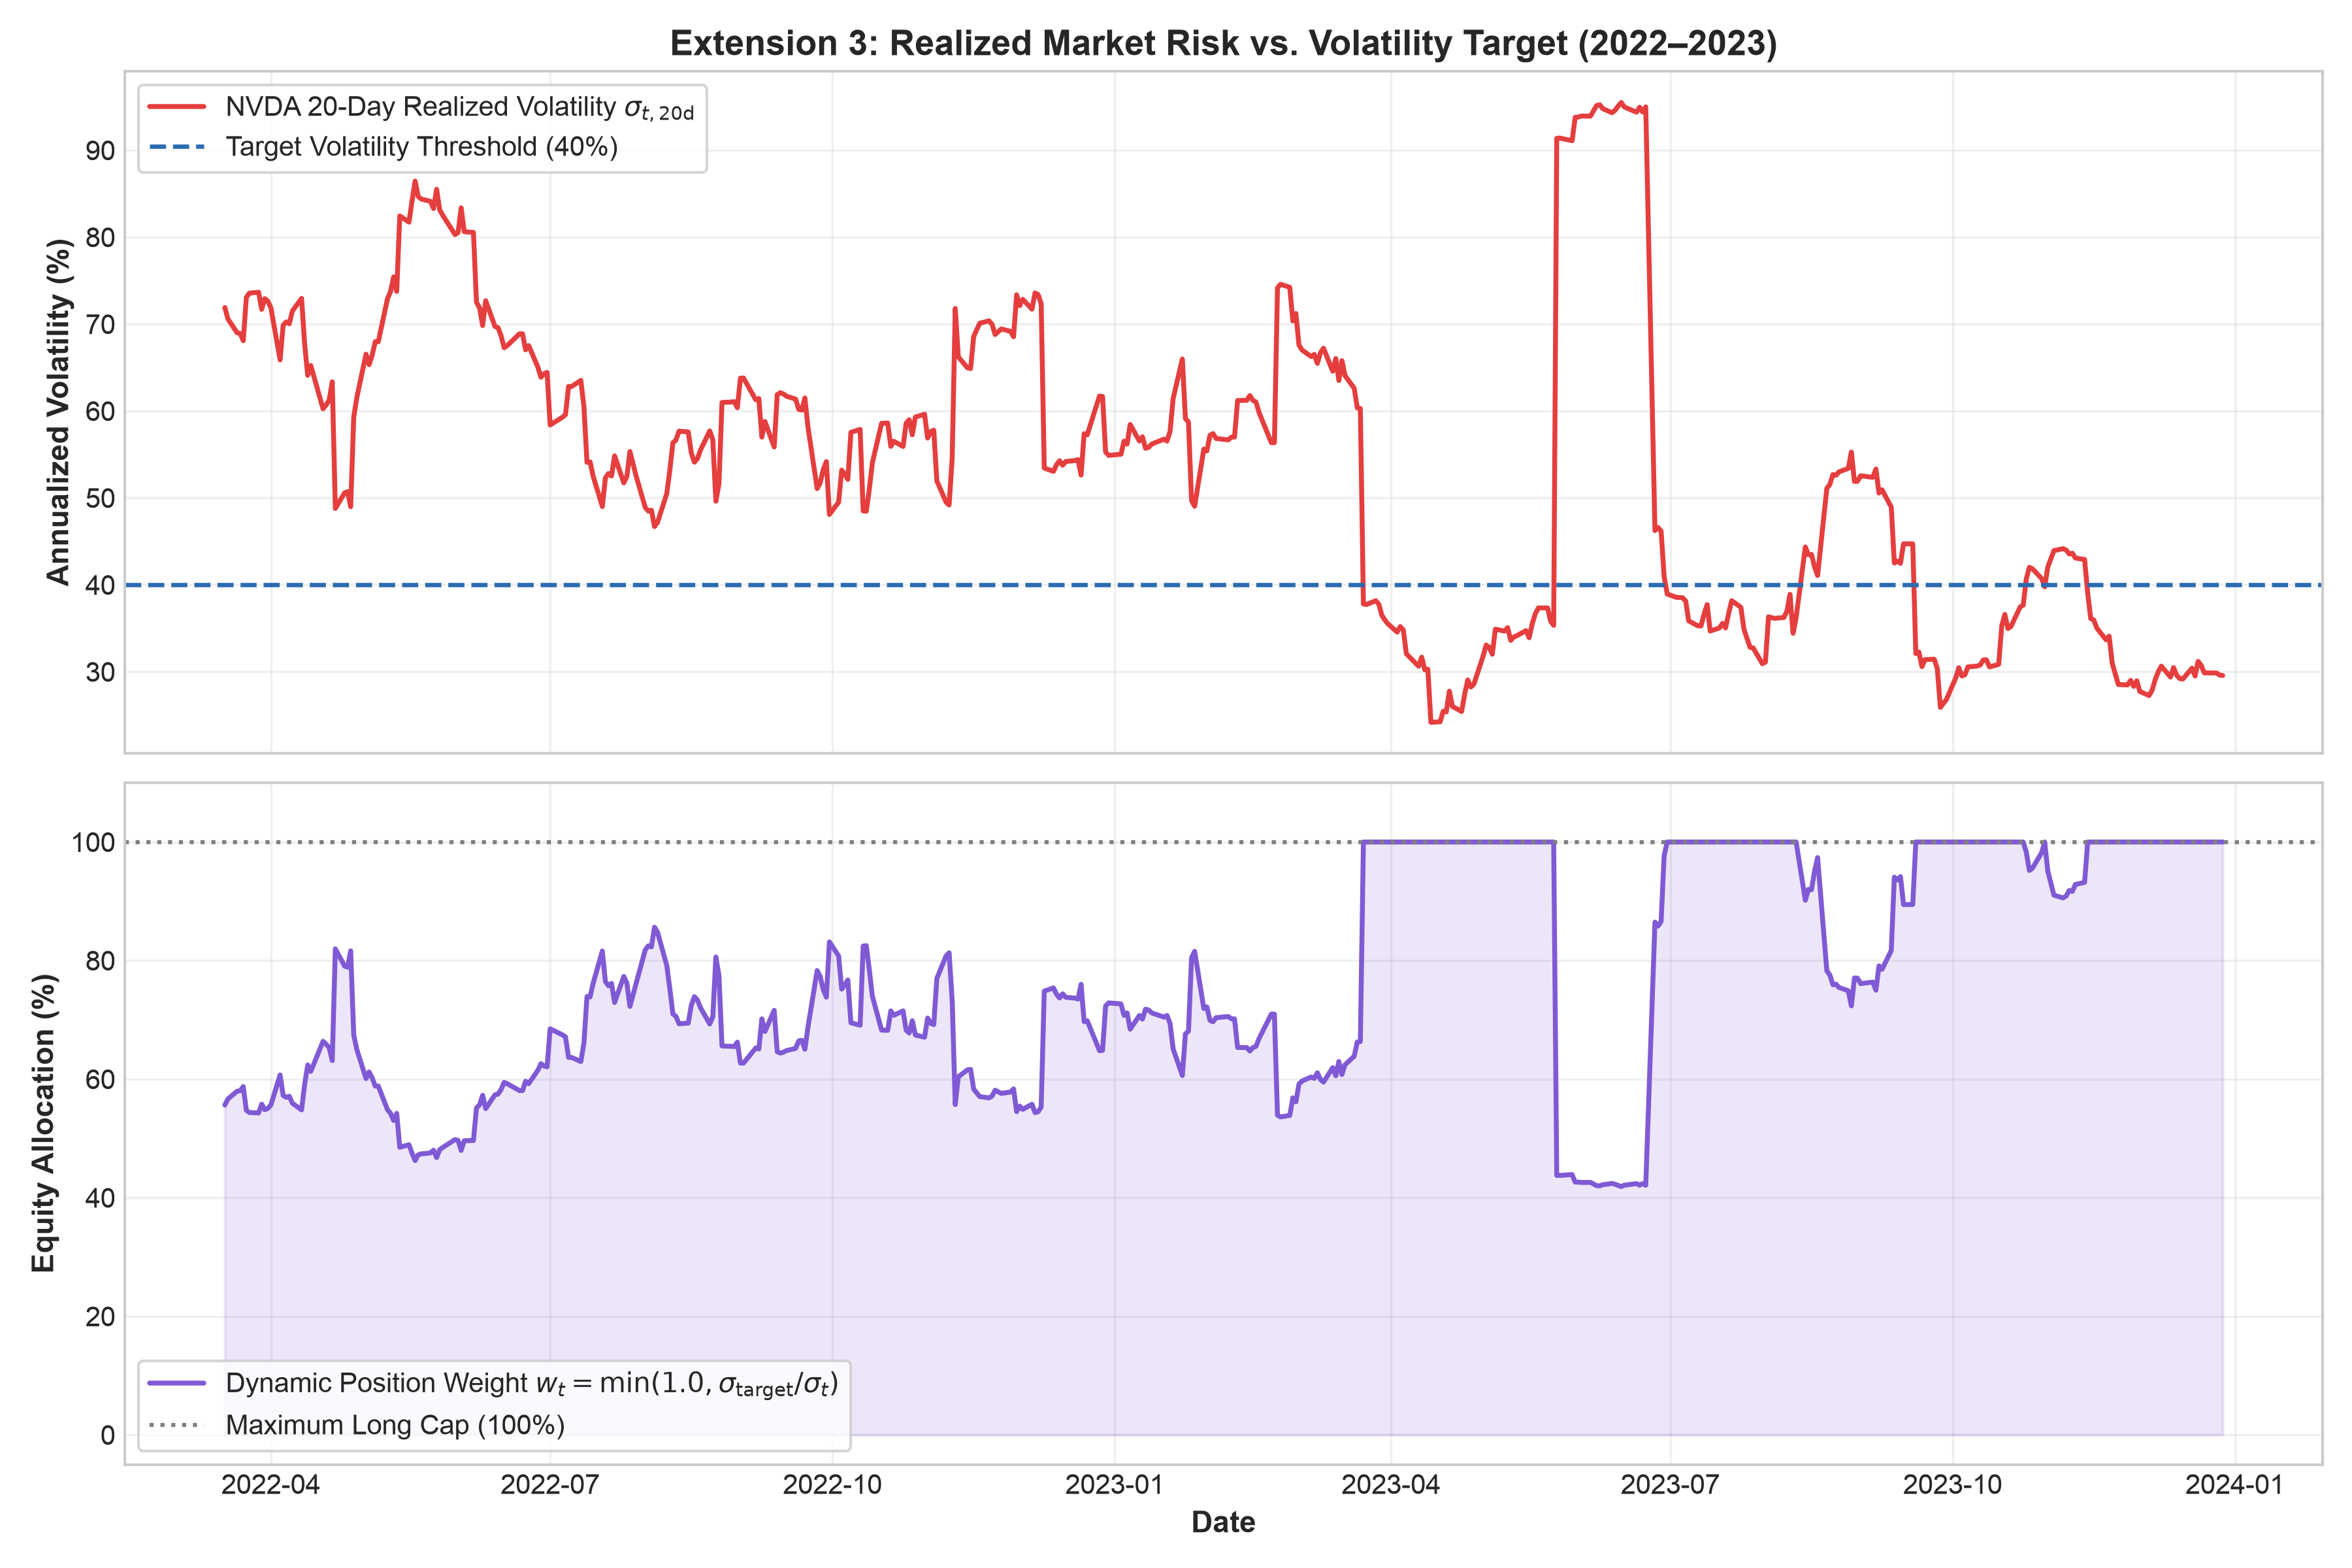
\includegraphics[width=0.82\textwidth]{ext3_volatility_allocation.png}
\caption{Trailing 20-day realized volatility vs.\ the 40\% target (top) and resulting portfolio weight $w_t$ (bottom).}
\label{fig:ext3_alloc}
\end{figure}

Table~\ref{tab:ablation} evaluates Strategy 3 across five target volatility levels ($\sigma_{\text{target}} \in \{20\%, 30\%, 40\%, 50\%, 60\%\}$).

\begin{table}[H]
\centering
\small
\setlength{\tabcolsep}{4.5pt}
\caption{Sensitivity of Strategy 3 to Target Volatility ($\sigma_{\text{target}}$) Across 449 Test Days.}
\label{tab:ablation}
\begin{tabularx}{\textwidth}{c R R R R R R}
\toprule
\textbf{Target Volatility} & \textbf{Ann.\ Return} & \textbf{CAGR} & \textbf{Ann.\ Vol} & \textbf{Sharpe} & \textbf{MaxDD} & \textbf{Turnover} \\
\midrule
20\% & 26.12\% & 25.31\% & 22.63\% & 1.15 & $-23.23\%$ & 4.25 \\
30\% & 38.67\% & 37.12\% & 33.75\% & 1.15 & $-33.33\%$ & 5.52 \\
\textbf{40\% (Baseline)} & \textbf{47.63\%} & \textbf{44.68\%} & \textbf{42.14\%} & \textbf{1.13} & \textbf{-42.45\%} & \textbf{5.10} \\
50\% & 51.51\% & 45.46\% & 48.46\% & 1.06 & $-50.71\%$ & 5.00 \\
60\% & 53.03\% & 43.88\% & 52.68\% & 1.01 & $-57.69\%$ & 2.85 \\
\bottomrule
\end{tabularx}
\end{table}

Table~\ref{tab:ablation} illustrates the risk-return trade-off across target levels:
\begin{itemize}
    \item \textbf{Lower Targets (20\%, 30\%):} Maintain large cash positions, achieving slightly higher Sharpe ratios (1.15) and smaller drawdowns ($-23.23\%$ and $-33.33\%$), but lower compound growth (25.31\% and 37.12\% CAGR) than Buy \& Hold (42.28\%).
    \item \textbf{Higher Targets (50\%, 60\%):} A 50\% target increases CAGR by 0.78 percentage points over the 40\% baseline (45.46\% vs.\ 44.68\%), but deepens maximum drawdown by 8.26 percentage points ($-50.71\%$ vs.\ $-42.45\%$) and reduces the Sharpe ratio to 1.06. At 60\%, higher variance drag lowers CAGR to 43.88\%.
    \item \textbf{Baseline Target (40\%):} Provides a balanced trade-off, exceeding Buy \& Hold CAGR while reducing maximum drawdown by 18.35 percentage points. Moreover, Sharpe ratios remain stable between 1.06 and 1.15 across the 20\%--50\% range.
\end{itemize}

\subsection{Trading Costs and Execution Robustness}
\label{sec:res_tradeoff}

Figure~\ref{fig:risk_return} plots annualized return against annualized volatility for all strategies and benchmarks. Both Strategy 2a and Strategy 3 achieve higher return per unit of risk than passive NVDA Buy \& Hold. Because annual transaction costs equal $\text{Turnover} \times 0.10\%$, Strategy 1's turnover of 39.85 reduced annual returns by 3.99\%, whereas Strategy 2a's turnover of 2.81 cost only 0.28\% per year.

\begin{figure}[H]
\centering
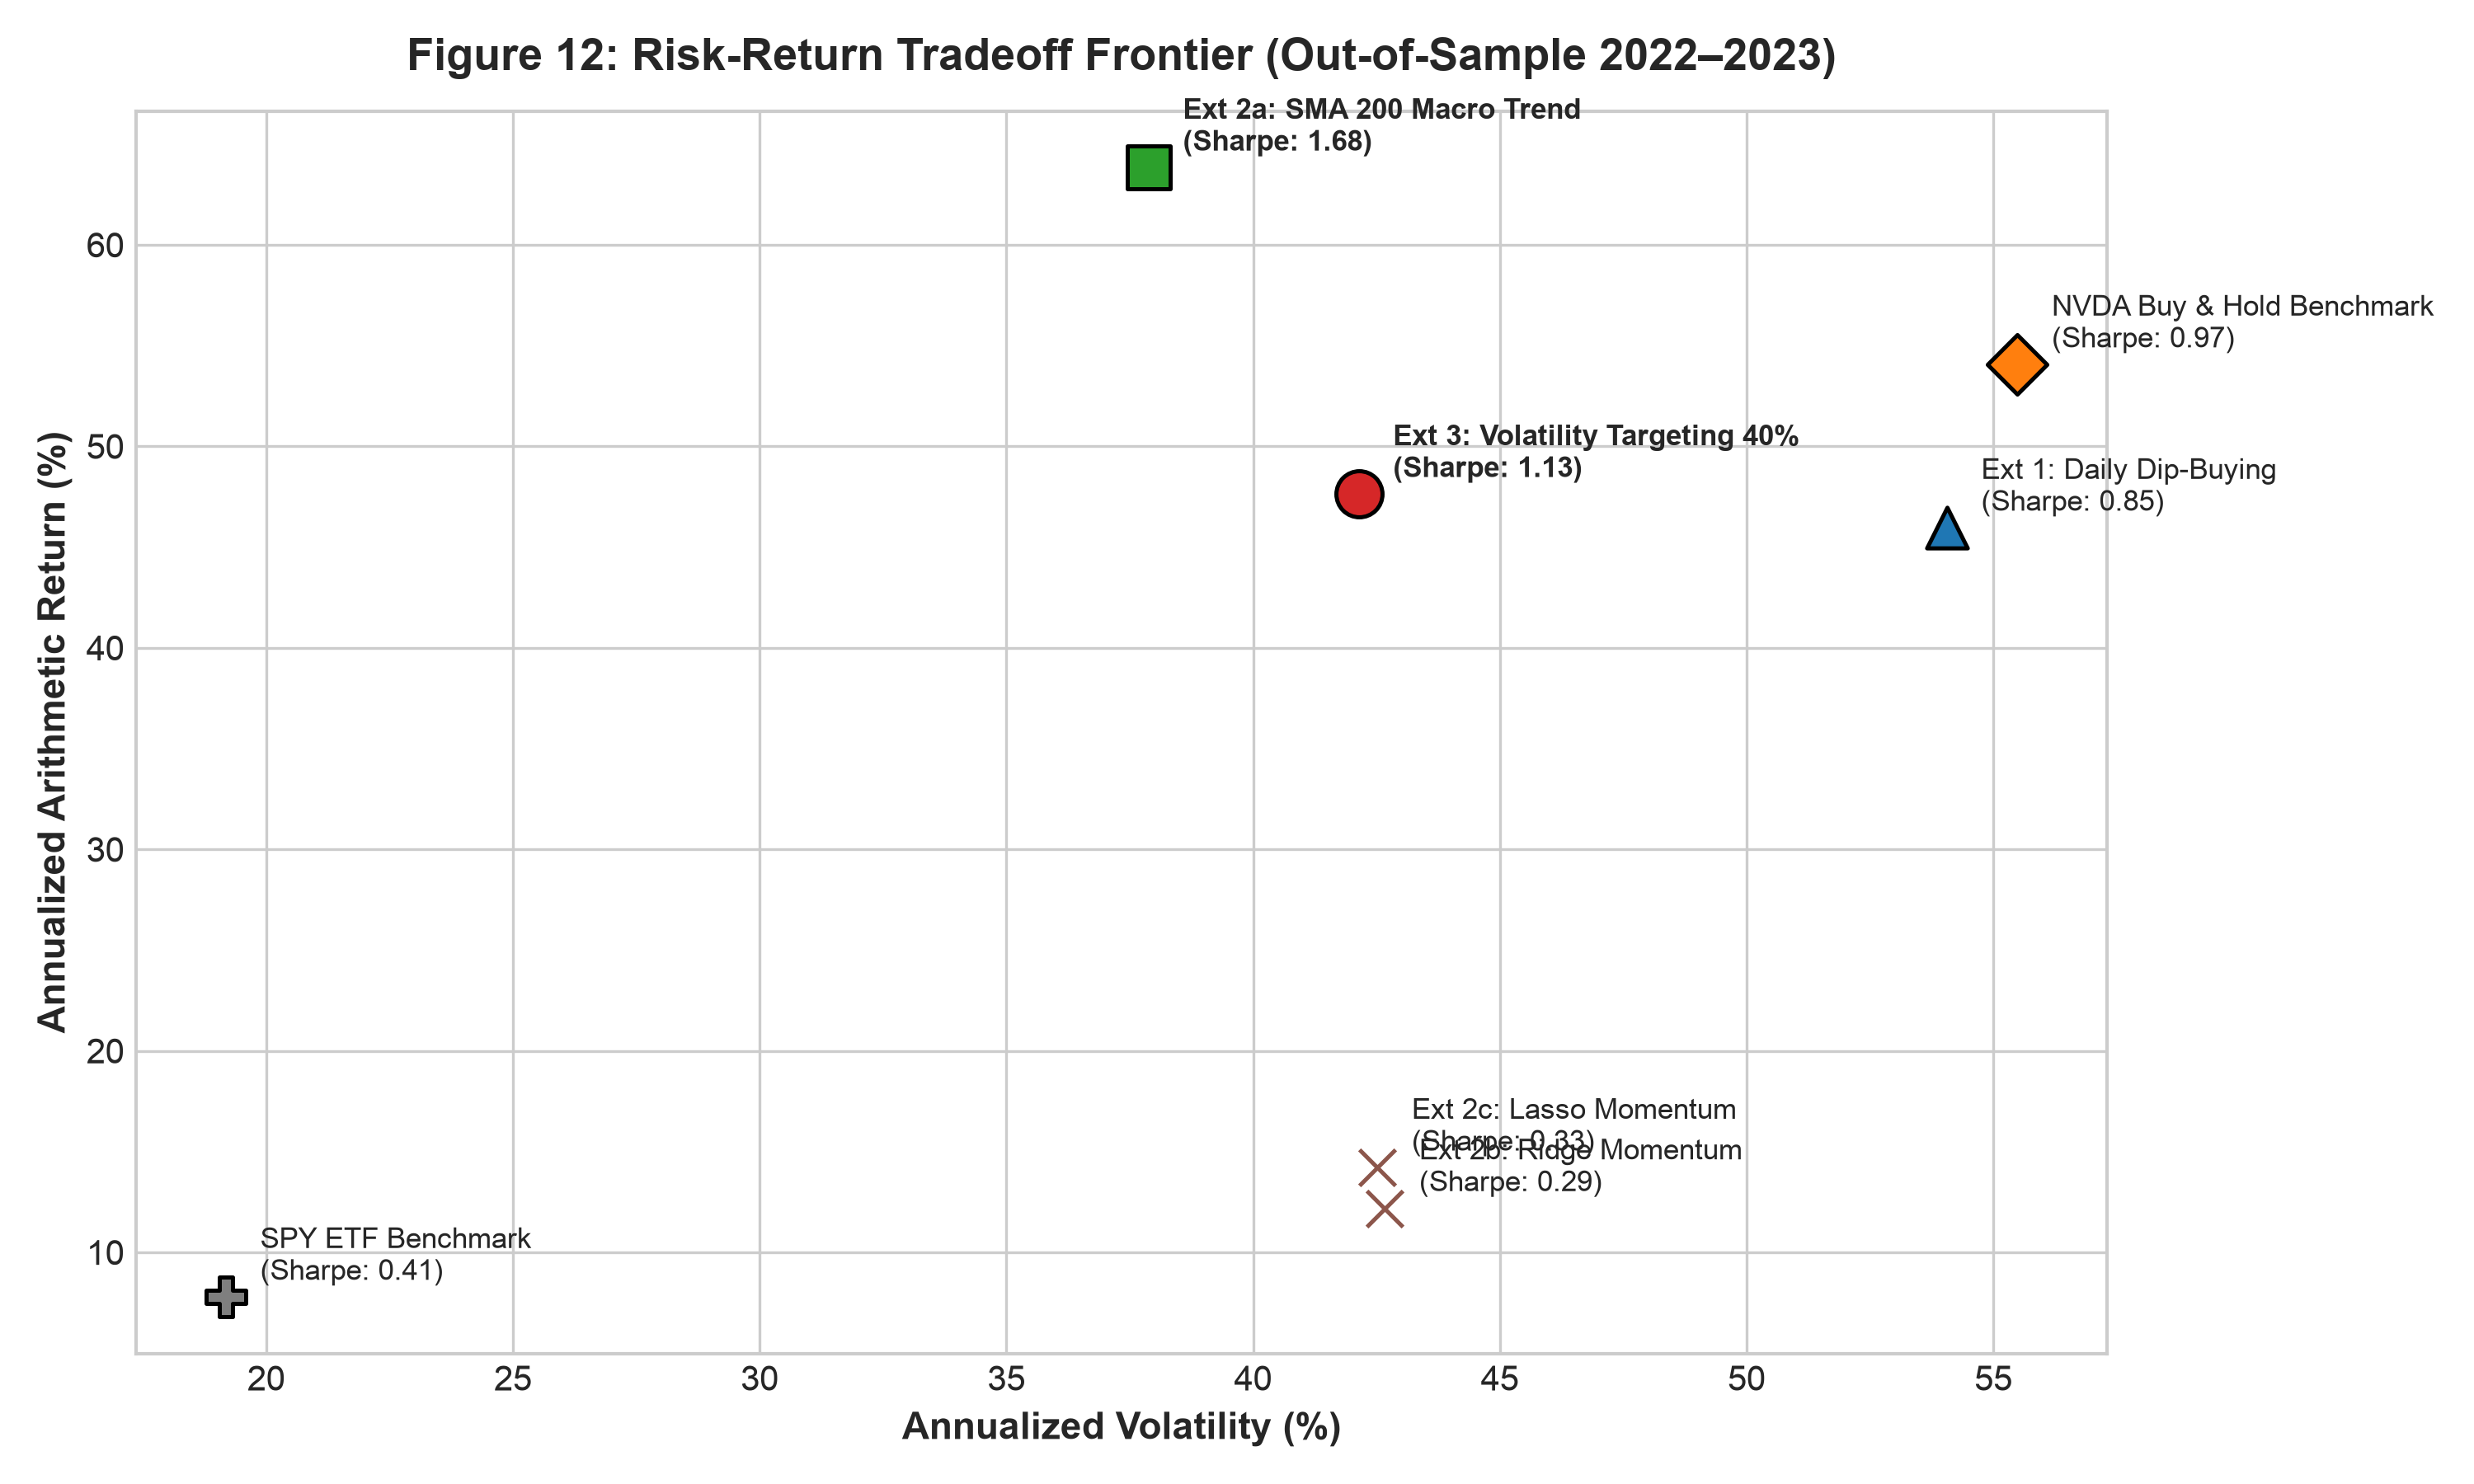
\includegraphics[width=0.72\textwidth, trim=0 26bp 0 0, clip]{consolidated_risk_return_tradeoff.png}
\caption{Annualized return vs.\ annualized volatility across strategies and benchmarks (449 test days).}
\label{fig:risk_return}
\end{figure}

To verify that the main findings do not depend on executing at the same day's close ($w_t \cdot R_{t+1}$), Table~\ref{tab:lag_audit} reports results under a one-day execution lag ($w_{t-1} \cdot R_{t+1}$), where signals computed at day $t-1$ are executed at day $t$ close.

\begin{table}[H]
\centering
\footnotesize
\setlength{\tabcolsep}{3.5pt}
\caption{Sensitivity to a One-Day Execution Lag ($w_{t-1} \cdot R_{t+1}$, 449 Test Days, Net of 10 bps Costs).}
\label{tab:lag_audit}
\begin{tabularx}{\textwidth}{l R R R R R}
\toprule
\textbf{Strategy / Benchmark (1-Day Lagged)} & \textbf{Ann.\ Return} & \textbf{CAGR} & \textbf{Ann.\ Vol} & \textbf{Sharpe} & \textbf{MaxDD} \\
\midrule
\textbf{Strategy 2a: 200-Day SMA Trend (Lag-1)} & \textbf{51.83\%} & \textbf{56.91\%} & \textbf{37.59\%} & \textbf{1.38} & \textbf{-30.22\%} \\
\textbf{Strategy 3: Volatility Targeting 40\% (Lag-1)} & \textbf{43.97\%} & \textbf{42.32\%} & \textbf{42.27\%} & \textbf{1.04} & \textbf{-44.65\%} \\
Strategy 2c: Lasso Momentum (Lag-1) & 34.61\% & 29.72\% & 42.00\% & 0.82 & $-41.02\%$ \\
Strategy 2b: Ridge Momentum (Lag-1) & 29.70\% & 23.29\% & 42.42\% & 0.70 & $-43.21\%$ \\
Strategy 1: Mean Reversion Ridge (Lag-1) & 35.83\% & 24.17\% & 53.83\% & 0.67 & $-67.57\%$ \\
\midrule
\textit{NVDA Buy \& Hold Benchmark} & 54.06\% & 42.28\% & 55.49\% & 0.97 & $-60.80\%$ \\
\textit{SPY ETF Benchmark} & 7.78\% & 5.48\% & 19.18\% & 0.41 & $-22.09\%$ \\
\bottomrule
\end{tabularx}
\end{table}

Under a full one-day execution lag, Strategy 2a still achieves a Sharpe ratio of 1.38, a CAGR of 56.91\%, and half the maximum drawdown of Buy \& Hold ($-30.22\%$ vs.\ $-60.80\%$). Strategy 3 also maintains a higher Sharpe ratio (1.04 vs.\ 0.97) and slightly higher CAGR (42.32\% vs.\ 42.28\%) than Buy \& Hold, confirming that the strategy ranking holds when same-day close execution is removed.

% =====================================================================
% 7. DISCUSSION
% =====================================================================
\section{Discussion}
\label{sec:discussion}

\subsection{Why Trend Following Worked}
Strategy 2a changed positions only four times across the 449-day test period:
\begin{itemize}
    \item 17 March 2022: Entered test window 100\% long.
    \item 7 April 2022: Exited to 100\% cash at \$242.67 when NVDA closed below its 200-day moving average.
    \item 12--15 December 2022: Briefly entered and exited during a short-lived breakout above the 200-day average.
    \item 13 January 2023: Re-entered 100\% long at \$169.59 as NVDA moved back above the 200-day average.
\end{itemize}

Staying in cash from April 2022 to January 2023 protected the portfolio when NVDA fell to a low of \$112.27 on 14 October 2022. Although the 200-day rule missed the initial rebound from the October bottom to the January re-entry, avoiding the bulk of the 2022 collapse outweighed the delayed re-entry, raising the Sharpe ratio from 0.97 to 1.68.

\subsection{Benefits and Limits of Volatility Targeting}
Strategy 3 illustrates how reducing return variance can improve compound growth ($g \approx \mu - \frac{1}{2}\sigma^2$). Even though passive NVDA had a higher arithmetic annual return (54.06\% vs.\ 47.63\%), Strategy 3 achieved a higher compound annual growth rate (44.68\% vs.\ 42.28\%) by lowering annualized volatility from 55.49\% to 42.14\%.

At the same time, volatility targeting has two practical trade-offs:
\begin{enumerate}
    \item \textbf{Partial Bear-Market Exposure:} Unlike a binary trend filter that moves fully to cash, volatility targeting remains partially invested during downturns. Its average equity weight in 2022 was 65.3\%, leading to a $-42.45\%$ maximum drawdown.
    \item \textbf{Symmetric Volatility Response:} Because standard deviation treats positive and negative returns equally, large positive price jumps (such as the 24.4\% post-earnings surge on 25 May 2023) increase trailing volatility and temporarily reduce equity exposure during bull markets.
\end{enumerate}

\subsection{Why Mean Reversion Underperformed}
Strategy 1 generated an annualized return of 45.96\% and a Sharpe ratio of 0.85, outperforming the SPY benchmark (0.41) but trailing NVDA Buy \& Hold (0.97) with a $-59.40\%$ maximum drawdown. Two factors explain this result:
\begin{itemize}
    \item \textbf{Buying Into Sustained Downtrends:} During the 2022 interest-rate tightening cycle, dips below the 10-day and 20-day moving averages triggered buy signals, but prices continued to fall rather than reverting to the mean.
    \item \textbf{High Turnover Costs:} Rebalancing on daily signals generated an annualized turnover of 39.85, reducing annual returns by 3.99\% at a 10 bps transaction cost.
\end{itemize}
Thus, short-term dip-buying requires a broader trend filter to avoid accumulating losses during multi-month bear markets.

\subsection{Limitations}
\label{sec:limits}
Several limitations should be considered when interpreting these findings:
\begin{enumerate}
    \item \textbf{Execution Timing:} The baseline backtest computes signals from the closing price $P_t$ and assumes execution at that same close. In live trading, market-on-close orders must be submitted before the 16:00 EST closing auction, and transaction costs alone do not eliminate this timing overlap. Live implementation would instead execute at the next day's open ($P_{t+1}^{\text{open}}$). Table~\ref{tab:lag_audit} shows that delaying execution by a full trading day ($P_{t+1}$ close) reduces Strategy 2a's Sharpe ratio from 1.68 to 1.38 and Strategy 3's from 1.13 to 1.04, while preserving their outperformance over Buy \& Hold (0.97).
    \item \textbf{Multiple Testing:} Comparing five strategy variants on the same 449-day holdout period introduces selection bias~\cite{white2000, harvey2016}. Selecting the best-performing rule after observing test results overstates expected future performance.
    \item \textbf{Sample Length:} The 449-day out-of-sample window (1.78 years) covers one major downturn (2022) and one major rally (2023), leaving Sharpe ratio estimates subject to finite-sample uncertainty~\cite{lo2002}.
    \item \textbf{Single-Asset Scope:} Results are derived from NVDA, a high-growth, high-volatility technology stock, and may not generalize to broader or lower-volatility equity portfolios.
    \item \textbf{Zero Risk-Free Rate and Cash Yield Assumption:} The backtest assumes uninvested cash ($1 - w_t$) earns 0\% interest and computes Sharpe ratios using $R_f = 0$~\cite{sharpe1994}. Incorporating prevailing 2022--2023 US Treasury bill yields (4--5\%) would have two distinct effects: (a) crediting interest on cash balances $(1 - w_t)R_{f,t}$ would increase the total return and CAGR of strategies that held cash during the 2022 downturn (such as Strategy 2a and Strategy 3), whereas (b) deducting $R_f > 0$ in the Sharpe ratio numerator $(R_{\text{ann}} - R_f)/\sigma_{\text{ann}}$ would lower excess return Sharpe ratios across all strategies.
\end{enumerate}

% =====================================================================
% 8. CONCLUSION
% =====================================================================
\section{Conclusion}
\label{sec:conclusion}

\subsection{Hypothesis Evaluation}
Based on the 449 out-of-sample trading days for NVDA from March 2022 to December 2023, the three hypotheses are evaluated as follows. Because the study examines a single stock over one bear-to-bull cycle, these conclusions apply to this empirical sample rather than all equity markets:
\begin{enumerate}
    \item \textbf{H1 (Mean Reversion): Not Supported Out-of-Sample.} In the training sample, Ridge regression learned negative coefficients on same-day returns (\texttt{Ret\_0}) and moving-average distances (\texttt{Dist\_MA10}, \texttt{Dist\_MA20}), which is directionally consistent with short-term reversal. However, in-sample coefficient signs alone do not establish out-of-sample predictive power or trading profitability. On the holdout test set, predictive accuracy was negative ($\text{OOS } R^2 = -0.00245$ vs.\ zero and $-0.00603$ vs.\ the training mean), and repeated dip-buying during the 2022 bear market produced a $-59.40\%$ maximum drawdown and a lower Sharpe ratio (0.85) than passive NVDA Buy \& Hold (0.97).
    \item \textbf{H2 (Trend Following): Supported for the 200-Day SMA Rule.} Conditioning exposure on the 200-day moving average avoided most of the 2022 downturn, achieving the highest Sharpe ratio (1.68) and lowest maximum drawdown ($-19.30\%$) in the test sample. By contrast, fitted Ridge and Lasso momentum models were sensitive to the exact training split date.
    \item \textbf{H3 (Volatility Targeting): Supported.} Scaling position sizes inversely to 20-day realized volatility reduced variance drag, increasing CAGR from 42.28\% (Buy \& Hold) to 44.68\% while reducing maximum drawdown from $-60.80\%$ to $-42.45\%$.
\end{enumerate}

\subsection{Key Findings}
\begin{itemize}
    \item \textbf{Simple Rules Outperformed Fitted Models:} A parameter-free 200-day moving average filter outperformed regularized regression models trained on noisy daily returns.
    \item \textbf{Volatility Control Improved Compounding:} Lowering annualized volatility by 13.35 percentage points enabled Strategy 3 to achieve higher compound growth than unhedged buy-and-hold despite a lower arithmetic mean return.
    \item \textbf{Turnover Directly Impacts Net Returns:} At 10 bps per trade, daily rebalancing cost Strategy 1 nearly 4\% per year, whereas low-turnover trend following lost less than 0.3\% per year to trading costs.
\end{itemize}

\subsection{Proposed Combined Strategy}
Because the three strategies operate at complementary horizons, they can be combined into a unified rule for future research:
\begin{equation}
w_{t+1}^* = \underbrace{\mathbb{I}(P_t > \text{SMA}_{200,t})}_{\text{Trend Filter}} \times \underbrace{\min\left(1.0, \frac{\sigma_{\text{target}}}{\sigma_{t, 20\text{d}}}\right)}_{\text{Volatility Scaling}} \times \underbrace{\mathbb{I}(\hat{y}_t^{\text{Ridge}} > 0)}_{\text{Short-Term Entry Filter}}
\end{equation}
This composite rule is a conceptual extension rather than a backtested model in Table~\ref{tab:master_showdown}, pairing 200-day regime filtering with volatility-scaled sizing and short-term entry timing.

% =====================================================================
% 9. REFERENCES
% =====================================================================
\newpage
\addcontentsline{toc}{section}{References}
\begin{thebibliography}{99}
\small
\setlength{\itemsep}{0.25em}

\bibitem{hurst1951} H. E. Hurst, ``Long-term storage capacity of reservoirs,'' \textit{Transactions of the American Society of Civil Engineers}, vol. 116, no. 1, pp. 770--799, 1951.

\bibitem{campbell2008} J. Y. Campbell and S. B. Thompson, ``Predicting excess stock returns out of sample: Can anything beat the historical average?,'' \textit{The Review of Financial Studies}, vol. 21, no. 4, pp. 1509--1531, 2008.

\bibitem{jegadeesh1990} N. Jegadeesh, ``Evidence of predictable behavior of security returns,'' \textit{The Journal of Finance}, vol. 45, no. 3, pp. 881--898, 1990.

\bibitem{lehmann1990} B. N. Lehmann, ``Fads, martingales, and market efficiency,'' \textit{The Quarterly Journal of Economics}, vol. 105, no. 1, pp. 1--28, 1990.

\bibitem{lomackinlay1990} A. W. Lo and A. C. MacKinlay, ``When are contrarian profits due to stock market overreaction?,'' \textit{The Review of Financial Studies}, vol. 3, no. 2, pp. 175--205, 1990.

\bibitem{hoerl1970} A. E. Hoerl and R. W. Kennard, ``Ridge regression: Biased estimation for nonorthogonal problems,'' \textit{Technometrics}, vol. 12, no. 1, pp. 55--67, 1970.

\bibitem{moskowitz2012} T. J. Moskowitz, Y. H. Ooi, and L. H. Pedersen, ``Time series momentum,'' \textit{Journal of Financial Economics}, vol. 104, no. 2, pp. 228--250, 2012.

\bibitem{faber2007} M. T. Faber, ``A quantitative approach to tactical asset allocation,'' \textit{The Journal of Wealth Management}, vol. 9, no. 4, pp. 69--79, 2007.

\bibitem{tibshirani1996} R. Tibshirani, ``Regression shrinkage and selection via the lasso,'' \textit{Journal of the Royal Statistical Society: Series B (Methodological)}, vol. 58, no. 1, pp. 267--288, 1996.

\bibitem{chinco2019} A. M. Chinco, A. D. Clark-Joseph, and M. Ye, ``Sparse signals in the cross-section of returns,'' \textit{The Journal of Finance}, vol. 74, no. 1, pp. 449--492, 2019.

\bibitem{mandelbrot1963} B. Mandelbrot, ``The variation of certain speculative prices,'' \textit{The Journal of Business}, vol. 36, no. 4, pp. 394--419, 1963.

\bibitem{engle1982} R. F. Engle, ``Autoregressive conditional heteroscedasticity with estimates of the variance of United Kingdom inflation,'' \textit{Econometrica}, vol. 50, no. 4, pp. 987--1007, 1982.

\bibitem{moreira2017} A. Moreira and T. Muir, ``Volatility-managed portfolios,'' \textit{The Journal of Finance}, vol. 72, no. 4, pp. 1611--1644, 2017.

\bibitem{harvey2018} C. R. Harvey, E. Hoyle, R. Korgaonkar, S. Rattray, M. Sargaison, and O. Van Hemert, ``The impact of volatility targeting,'' \textit{The Journal of Portfolio Management}, vol. 45, no. 1, pp. 14--33, 2018.

\bibitem{sharpe1994} W. F. Sharpe, ``The Sharpe ratio,'' \textit{The Journal of Portfolio Management}, vol. 21, no. 1, pp. 49--58, 1994.

\bibitem{pedregosa2011} F. Pedregosa \textit{et al.}, ``Scikit-learn: Machine learning in Python,'' \textit{Journal of Machine Learning Research}, vol. 12, pp. 2825--2830, 2011.

\bibitem{fama1970} E. F. Fama, ``Efficient capital markets: A review of theory and empirical work,'' \textit{The Journal of Finance}, vol. 25, no. 2, pp. 383--417, 1970.

\bibitem{white2000} H. White, ``A reality check for data snooping,'' \textit{Econometrica}, vol. 68, no. 5, pp. 1097--1126, 2000.

\bibitem{harvey2016} C. R. Harvey, Y. Liu, and H. Zhu, ``\dots and the cross-section of expected returns,'' \textit{The Review of Financial Studies}, vol. 29, no. 1, pp. 5--68, 2016.

\bibitem{lo2002} A. W. Lo, ``The statistics of Sharpe ratios,'' \textit{Financial Analysts Journal}, vol. 58, no. 4, pp. 36--52, 2002.

\end{thebibliography}

% =====================================================================
% 10. APPENDIX
% =====================================================================
\newpage
\appendix
\section{Execution Commands and Terminal Verification}
\label{app:run}

All experiments can be reproduced directly from the project repository at \url{https://github.com/PokezardVGC/dsa5205-project-2}:

\begin{lstlisting}[language=bash]
# 1. Environment configuration
python3 -m venv .venv && source .venv/bin/activate
pip install -r requirements.txt

# 2. Automated test suite verification (6 unit tests)
python3 -m pytest tests/

# 3. Master Showdown: executes all 5 strategies on the aligned 449-day window
python3 scripts/run_consolidated_showdown.py

# 4. Individual module runners
python3 main.py                            # Strategy 1 standalone runner (Ridge Mean Reversion)
python3 scripts/run_extension2_momentum.py # Strategy 2 standalone runner (Trend and Momentum)
python3 src/strategy_volatility.py         # Strategy 3 standalone runner (Volatility Targeting)
\end{lstlisting}

\subsection*{Expected Output of Master Showdown Harness}
\begin{lstlisting}
===============================================================================================
Strategy / Benchmark                   | Ann. Ret  | CAGR      | Ann. Vol  | Sharpe  | MaxDD    | Turnover
-----------------------------------------------------------------------------------------------
Strategy 1: Daily Dip-Buying (Ridge)   |  45.96%   |  32.31%   |  54.06%   |   0.85  | -59.40%  |  39.85
Strategy 2a: 200d SMA Macro Trend      |  63.83%   |  70.36%   |  37.88%   |   1.68  | -19.30%  |   2.81
Strategy 2b: Ridge Momentum            |  12.19%   |   3.39%   |  42.67%   |   0.29  | -48.35%  |  30.31
Strategy 2c: Lasso Momentum            |  14.20%   |   5.56%   |  42.52%   |   0.33  | -44.61%  |  29.18
Strategy 3: Volatility Targeting 40%   |  47.63%   |  44.68%   |  42.14%   |   1.13  | -42.45%  |   5.10
NVDA Buy & Hold Benchmark              |  54.06%   |  42.28%   |  55.49%   |   0.97  | -60.80%  |   0.00
SPY ETF Benchmark                      |   7.78%   |   5.48%   |  19.18%   |   0.41  | -22.09%  |   0.00
===============================================================================================
\end{lstlisting}

\section{Core Reproducible Source Code}
\label{app:code}

\subsection*{Module 1: Feature Engineering Pipeline}
\noindent\textit{Source File: \texttt{src/features.py}}
\begin{lstlisting}[language=Python]
import pandas as pd
import numpy as np

def engineer_features(df):
    df['Return'] = df['Price'].pct_change()
    df['Ret_0'] = df['Return']
    df['Ret_Lag1'] = df['Return'].shift(1)
    df['Ret_Lag2'] = df['Return'].shift(2)
    df['Ret_Lag5'] = df['Price'].pct_change(5).shift(1)
    df['MA_10'] = df['Price'].rolling(window=10).mean()
    df['Dist_MA10'] = (df['Price'] - df['MA_10']) / df['MA_10']
    df['MA_20'] = df['Price'].rolling(window=20).mean()
    df['Dist_MA20'] = (df['Price'] - df['MA_20']) / df['MA_20']
    df['Target_Next_Return'] = df['Return'].shift(-1)
    df = df.replace([np.inf, -np.inf], np.nan).dropna()
    features = ['Ret_0', 'Ret_Lag1', 'Ret_Lag2', 'Ret_Lag5', 'Dist_MA10', 'Dist_MA20']
    df.loc[:, features] = df[features].clip(-0.5, 0.5)
    return df, features
\end{lstlisting}

\subsection*{Module 2: Ridge Regularization and Model Selection}
\noindent\textit{Source File: \texttt{src/model.py}}
\begin{lstlisting}[language=Python]
import pandas as pd
import numpy as np
from sklearn.linear_model import Ridge
from sklearn.preprocessing import StandardScaler
from sklearn.model_selection import TimeSeriesSplit

def train_and_select_model(df, features):
    X = df[features]
    y = df['Target_Next_Return'].clip(-0.5, 0.5)
    train_size = int(len(df) * 0.8)
    X_train_val, y_train_val = X.iloc[:train_size], y.iloc[:train_size]
    X_test = X.iloc[train_size:]
    
    tscv = TimeSeriesSplit(n_splits=5)
    best_alpha, best_score = None, -float('inf')
    for alpha in [0.1, 1.0, 10.0, 100.0, 1000.0]:
        scores = []
        for tr_idx, val_idx in tscv.split(X_train_val):
            scaler = StandardScaler()
            X_tr = scaler.fit_transform(X_train_val.iloc[tr_idx])
            X_val = scaler.transform(X_train_val.iloc[val_idx])
            m = Ridge(alpha=alpha).fit(X_tr, y_train_val.iloc[tr_idx])
            scores.append(m.score(X_val, y_train_val.iloc[val_idx]))
        if np.mean(scores) > best_score:
            best_score, best_alpha = np.mean(scores), alpha
            
    final_scaler = StandardScaler()
    X_tr_val_s = final_scaler.fit_transform(X_train_val)
    best_model = Ridge(alpha=best_alpha).fit(X_tr_val_s, y_train_val)
    preds = best_model.predict(final_scaler.transform(X_test))
    return best_model, preds, X_test.index
\end{lstlisting}

\subsection*{Module 3: Macro Trend and Regularized Momentum Filter}
\noindent\textit{Harness File: \texttt{scripts/run\_consolidated\_showdown.py}}
\begin{lstlisting}[language=Python]
import numpy as np
import pandas as pd
from sklearn.linear_model import Ridge, Lasso
from sklearn.preprocessing import StandardScaler

def run_extension2(df_raw, test_index, tc=0.0010):
    df_m = df_raw.copy()
    df_m['Return'] = df_m['Price'].pct_change()
    df_m['Target_Next_Return'] = df_m['Return'].shift(-1)
    df_m['SMA_50'] = df_m['Price'].rolling(50).mean()
    df_m['SMA_200'] = df_m['Price'].rolling(200).mean()
    df_m['Dist_SMA50'] = (df_m['Price'] - df_m['SMA_50']) / df_m['SMA_50']
    df_m['Dist_SMA200'] = (df_m['Price'] - df_m['SMA_200']) / df_m['SMA_200']
    df_m['Mom_10d'] = df_m['Price'].pct_change(10)
    df_m['Mom_20d'] = df_m['Price'].pct_change(20)

    # Strategy 2a: Non-parametric 200-day trend rule
    pos_2a = np.where(df_m.loc[test_index, 'Price'] > df_m.loc[test_index, 'SMA_200'], 1.0, 0.0)
    
    # ML Momentum setup (Ridge and Lasso)
    m_feat = ['Dist_SMA50', 'Dist_SMA200', 'Mom_10d', 'Mom_20d']
    train_m = df_m.loc[df_m.index < test_index[0]].dropna()
    scaler = StandardScaler().fit(train_m[m_feat])
    y_tr = train_m['Target_Next_Return'].clip(-0.5, 0.5)
    
    ridge_m = Ridge(alpha=10.0).fit(scaler.transform(train_m[m_feat]), y_tr)
    lasso_m = Lasso(alpha=1e-5, random_state=42, max_iter=10000).fit(scaler.transform(train_m[m_feat]), y_tr)
    pos_2b = np.where(ridge_m.predict(scaler.transform(df_m.loc[test_index, m_feat])) > y_tr.mean(), 1.0, 0.0)
    pos_2c = np.where(lasso_m.predict(scaler.transform(df_m.loc[test_index, m_feat])) > y_tr.mean(), 1.0, 0.0)
    return pos_2a, pos_2b, pos_2c
\end{lstlisting}

\subsection*{Module 4: Dynamic Volatility Targeting Strategy}
\noindent\textit{Source File: \texttt{src/strategy\_volatility.py}}
\begin{lstlisting}[language=Python]
import numpy as np
import pandas as pd

def compute_volatility_features(df, vol_window=20, target_vol=0.40, epsilon=1e-6):
    df_out = df.copy()
    df_out['Daily_Return'] = df_out['Price'].pct_change()
    df_out['Target_Next_Return'] = df_out['Daily_Return'].shift(-1)
    rolling_std = df_out['Daily_Return'].rolling(window=vol_window, min_periods=vol_window).std()
    df_out['Rolling_Vol_20d'] = rolling_std * np.sqrt(252)
    safe_vol = np.maximum(df_out['Rolling_Vol_20d'], epsilon)
    df_out['Target_Weight'] = target_vol / safe_vol
    df_out['Position'] = np.clip(df_out['Target_Weight'], 0.0, 1.0)
    return df_out
\end{lstlisting}

\end{document}
